%\documentclass[smalldemyvopaper,11pt,twoside,onecolumn,openright,extrafontsizes]{memoir}
\documentclass[20pt,twoside,openright,extrafontsizes,landscape]{memoir}
\usepackage{yfonts,color,hyperref}
\def\initdefault{yinit}
  \usepackage{fontspec}
%\usepackage[T1]{inputenc}
\usepackage{fontspec}
\usepackage[spanish]{babel}
\usepackage{xsavebox} %save content for repeated use
\usepackage{atbegshi} %insert material on every page
\usepackage[x11names,dvipsnames]{xcolor} 
\usepackage{wrapfig}  
\usepackage{tikz}
\usepackage[tmargin=3cm,bmargin=3cm,lmargin=1cm,rmargin=2cm]{geometry}
%\usepackage[margin=1cm]{geometry}% for screen preview
\usepackage{graphicx}
\setmainfont{juan_letra_reg}
%\DeclareFontFamily{LYG}{OldNewspaperTypes}{}
	
%\AtBeginShipout{
%	\AtBeginShipoutUpperLeft{\raisebox{-\height}{\xusebox{PageBGPicture}}}
%}
\tolerance=1
\emergencystretch=\maxdimen
\hyphenpenalty=10000
\hbadness=10000
\usetikzlibrary{calc}
\usepackage{relsize}
\tikzset{fontscale/.style = {font=\relsize{#1}}
}
\begin{document}
	\begin{Large}
\pagenumbering{gobble}
\noindent
		\begin{tikzpicture}[remember picture, overlay]
			\node [inner sep=0pt, minimum width=\paperwidth, minimum height=\paperheight] at (current page.center) {\includegraphics[width=\paperwidth,height=\paperheight,angle=0]{portada}};
		\end{tikzpicture}
\iffalse

\newpage
		\begin{tikzpicture}[remember picture, overlay]
	\node [inner sep=0pt, minimum width=\paperwidth, minimum height=\paperheight] at (current page.center) {\includegraphics[width=\paperwidth,height=\paperheight,angle=0]{presenta}};
\end{tikzpicture}
%\end{Large}
\begin{minipage}{.35\textwidth}
	\begin{large}
HOLA, MI NOMBRE ES OTTOKO, VIVO EN VILLA DEVOTO. 
SI BIEN PUEDE PARECERLES QUE LLEVO UNA VIDA APACIBLE Y HASTA UN TANTO PEREZOSA, 

VOY A 

CONTARLES 

LA ÚLTIMA 

DE MIS 

INTRÉPIDAS

 AVENTURAS.	
		
\end{large}
\end{minipage}	

\newpage
\begin{tikzpicture}[remember picture, overlay]
	\node [inner sep=0pt, minimum width=\paperwidth, minimum height=\paperheight] at (current page.center) {\includegraphics[width=\paperwidth,height=\paperheight,angle=0]{presenta2}};
	
	\node[text width=24cm,xshift=0cm,yshift=8cm] at (current page.center){PUEDE QUE ALGUIEN DESCONFÍE DE LOS RELATOS DE UN GATO NEGRO, $\ldots$ ¿QUIÉN NO HA ESCUCHADO DECIR QUE LOS GATOS NEGROS TRAEMOS MALA SUERTE? ¡PURAS PATRAÑAS! };	
	
		\node[text width=15cm,xshift=-4.5cm,yshift=1.6cm] at (current page.center){A VECES, REPETIR COSAS SIN PENSAR RESULTA FÁCIL Y CÓMODO. POR ESO, AÚN HOY HAY PERSONAS QUE CREEN QUE EL PLANETA TIERRA ES PLANO, QUE LA ASTROLOGÍA SIRVE PARA CONOCERSE, QUE EXISTEN EL MAL DE OJO Y LAS BRUJERÍAS$\ldots$ LOS HUMANOS };	
		\node[text width=24cm,xshift=0cm,yshift=-6cm] at (current page.center){
		SON CAPACES DE ÉSTAS Y TANTAS OTRAS SANDECES CUANDO NO TIENEN GANAS DE RAZONAR. 
		
		A MÍ ME GUSTA PENSAR, SERÁ PORQUE ES NECESARIO PARA SER UN BUEN CAZADOR FELINO.	YO YA DESDE CHIQUITO, PENSABA EN CÓMO ATRAPAR PALOMAS.};
	

\end{tikzpicture}
\newpage
\begin{tikzpicture}[remember picture, overlay]
	\node [inner sep=0pt, minimum width=\paperwidth, minimum height=\paperheight] at (current page.center) {\includegraphics[width=\paperwidth,height=\paperheight,angle=0]{paloma1}};
	
		\node[text width=15cm,xshift=-4.5cm,yshift=2cm] at (current page.center){¡PALOMAS! ALGUNOS CAMARADAS LAS LLAMAN RATAS DEL AIRE. ¡SÍ!, LOS GATOS CONOCEMOS A LOS MURCIÉLAGOS PERO HAY MUCHOS MENOS QUE PALOMAS EN LAS CIUDADES. 
			
			ÉSTAS AVES ADAPTARON SU PLUMAJE AL COLOR DEL CEMENTO DE LOS EDIFICIOS, DEL ASFALTO DE LAS CALLES, AUNQUE, PARA MÍ, IMITAN AL TINTE DE LA MUGRE.};	
\node[text width=5cm,yshift=9.5cm,xshift=8cm] at (current page.center){¡UH! ¡UH! ¡UH!};
	
	
\end{tikzpicture}
\newpage
\begin{tikzpicture}[remember picture, overlay]
	\node [inner sep=0pt, minimum width=\paperwidth, minimum height=\paperheight] at (current page.center) {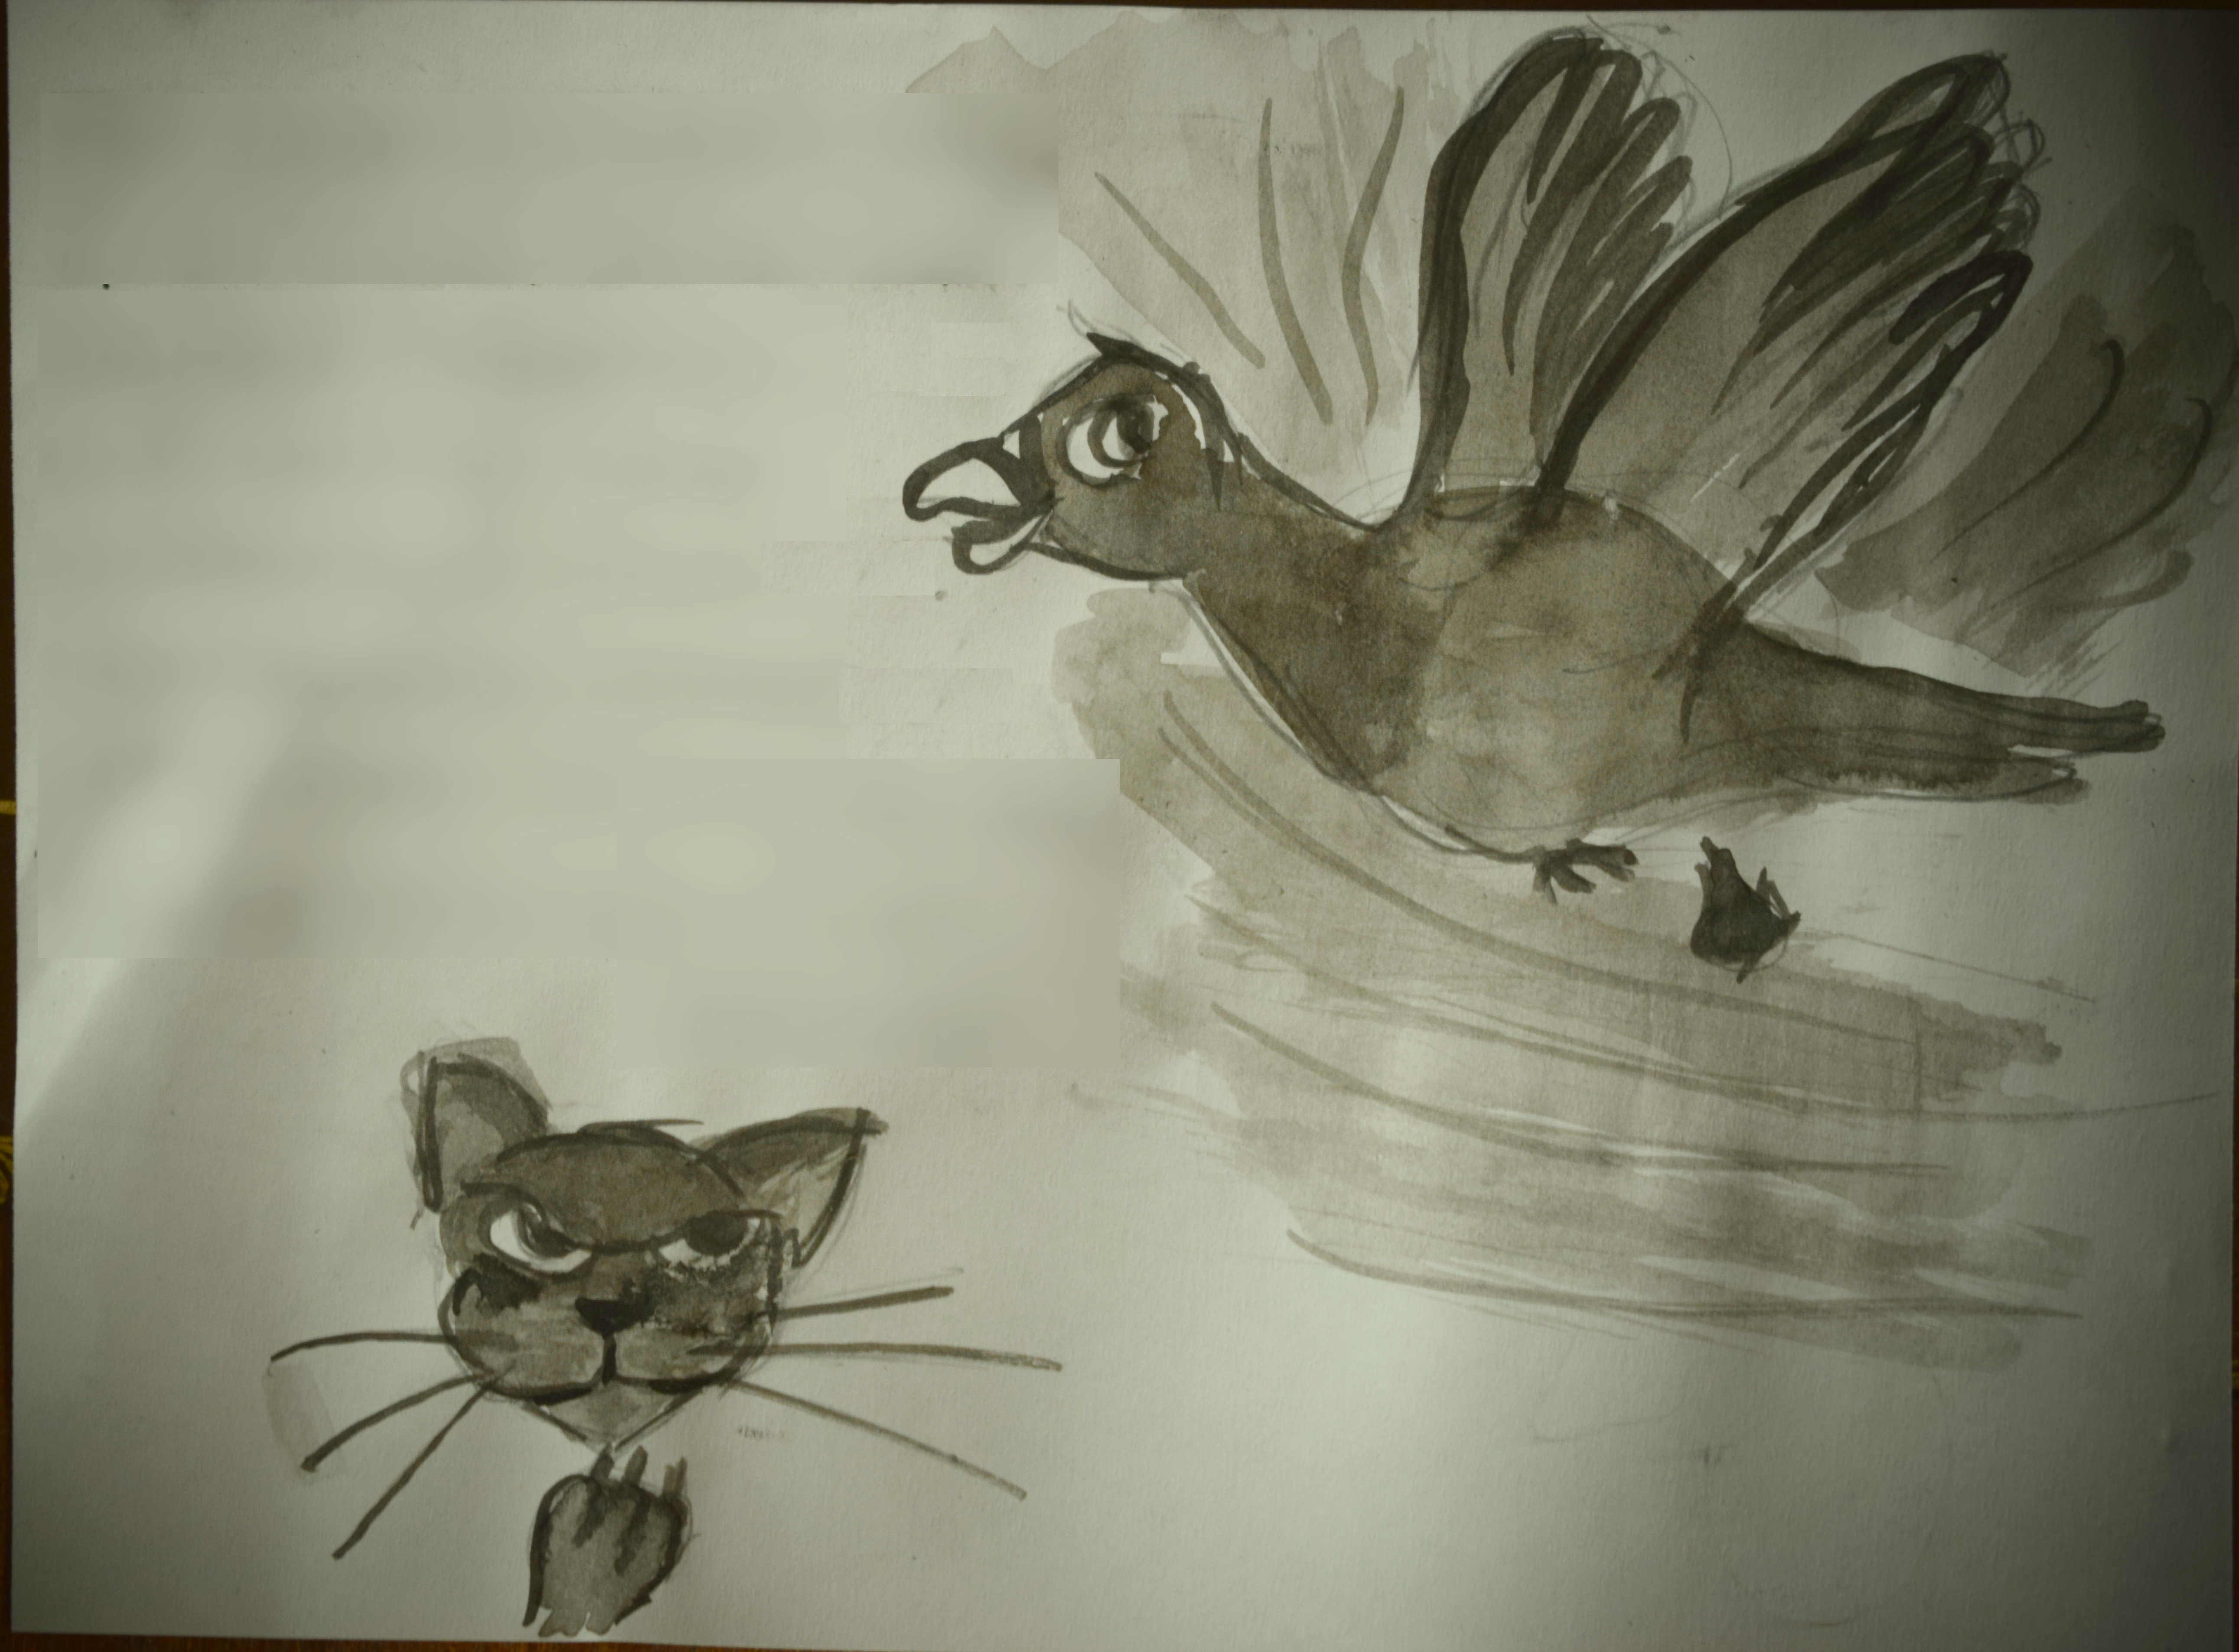
\includegraphics[width=\paperwidth,height=\paperheight,angle=0]{paloma2}};
	
		\node[text width=15cm,xshift=-4.5cm,yshift=2cm] at (current page.center){SI BIEN DE MIRADA TORPE Y DE CAMINAR MUY POCO ELEGANTE, 
			\newline\newline
			
			RECONOZCO QUE SON MUY ASTUTAS PARA EMPRENDER EL VUELO.
			
			TAMBIÉN ADMIRO ALGUNA DE SUS HABILIDADES MUY PRÁCTICAS PARA LA VIDA COTIDIANA, ¡ Y SIN PIEDRITAS!};	
	
	
	
\end{tikzpicture}

\newpage
\begin{tikzpicture}[remember picture, overlay]
	\node [inner sep=0pt, minimum width=\paperwidth, minimum height=\paperheight,opacity=0.9] at (current page.center) {\includegraphics[width=\paperwidth,height=\paperheight,angle=0]{comiendo}};
	
		\node[text width=26cm,xshift=0cm,yshift=0cm] at (current page.center){PUES ME ENCONTRABA MUY TRANQUILO UNA MAÑANA COMIENDO MIS DELICIOSAS CROQUETAS PARA GATO (A VECES CONFIESO QUE ME HE DESAYUNADO CUCARACHAS PERO ESA ES OTRA HISTORIA) CUANDO ESCUCHÉ DESDE EL PATIO EL ARRULLO DE UNAS PALOMAS.
			\newline\newline\newline
						\newline\newline\newline
			
			ESTABA ABIERTO EL VENTANAL Y DECIDÍ DAR UN VISTAZO . ALLÍ ESTABAN, CHARLANDO ENTRE ELLAS. CON MI HABITUAL CURIOSIDAD FELINA, ME ACERQUÉ UN POCO HACIA DONDE ESTABAN.
		
	¡CASI AL INSTANTE DESCUBRÍ QUE ME HABÍAN ENGAÑADO! PUES UNA INSOLENTE AVE, HABÍA APROVECHADO MI DISTRACCIÓN PARA ~~~~SAQUEAR MI PLATO.};	
		
	
	
\end{tikzpicture}
\newpage
\begin{tikzpicture}[remember picture, overlay]
	\node [inner sep=0pt, minimum width=\paperwidth, minimum height=\paperheight] at (current page.center) {\includegraphics[width=\paperwidth,height=\paperheight,angle=0]{salto_paloma}};
	
		\node[text width=14cm,xshift=-4cm,yshift=0cm] at (current page.center){SI BIEN FUE UNO
			
			 DE MIS MEJORES
			 
			  SALTOS, NO CONSEGUÍ 
			  
			  ATRAPARLA. ¡UN GATO JOVEN COMO YO TENDRÍA MÁS OPORTUNIDADES EN EL FUTURO! 
			  
			  DESDE LO ALTO DEL MURO, LAS 
			  
			  PALOMAS SE BURLABAN DESCARADAMENTE. 
			  
			  SÍ, O AL MENOS ESO PENSÉ DE LOS MÚLTIPLES 'UH-UH-UH' QUE LLEGABAN A MIS OÍDOS. ALGO FURIOSO, DECIDÍ DARLES UNA LECCIÓN DE HUMILDAD.
};	
		
	
	
\end{tikzpicture}

\newpage
\begin{tikzpicture}[remember picture, overlay]
	\node [inner sep=0pt, minimum width=\paperwidth, minimum height=\paperheight] at (current page.center) {\includegraphics[width=\paperwidth,height=\paperheight,angle=0]{salto_paloma}};
	
		\node[text width=14cm,xshift=-4cm,yshift=0cm] at (current page.center){SI BIEN FUE UNO
			
			DE MIS MEJORES
			
			SALTOS, NO CONSEGUÍ 
			
			ATRAPARLA. ¡UN GATO JOVEN COMO YO TENDRÍA MÁS OPORTUNIDADES EN EL FUTURO! 
			
			DESDE LO ALTO DEL MURO, LAS 
			
			PALOMAS SE BURLABAN DESCARADAMENTE. 
			
			SÍ, O AL MENOS ESO PENSÉ DE LOS MÚLTIPLES 'UH-UH-UH' QUE LLEGABAN A MIS OÍDOS. ALGO FURIOSO, DECIDÍ DARLES UNA LECCIÓN DE HUMILDAD.
		};	
		
	
	
\end{tikzpicture}

\newpage
\begin{tikzpicture}[remember picture, overlay]
	\node [inner sep=0pt, minimum width=\paperwidth, minimum height=\paperheight] at (current page.center) {\includegraphics[width=\paperwidth,height=\paperheight,angle=0]{reflexion}};
	
		\node[text width=22cm,xshift=-1cm,yshift=0cm] at (current page.center){TOMÉ CORAJE Y SEGUÍ TREPANDO. UTILICÉ LA ESQUINA 
			
			QUE FORMAN LAS PAREDES  
			
			Y FINALMENTE ALCANCÉ
			
			 TODO LO ALTO 		DEL MURO.
			 
			  HAY ALLÍ UNA 		ESPECIE 
			  
			  DE CANTERO Y ME
			
			 METÍ DENTRO DE LO QUE
			 
			 ES  UNA CANALETA. ES DONDE
			 
			  CORRE  			 EL AGUA QUE MIRO CAER
			  
			   FASCINADO   LOS DÍAS DE LLUVIA.
			   
			    DESDE ESE LUGAR ESTABA PODÍA VER TODO EL 
			    
			    PATIO, DONDE SOLEMOS JUGAR. MI ESFUERZO RESULTÓ TAN GRANDE QUE NECESITÉ DESCANSAR UN RATO.
		};	
		
	
	
\end{tikzpicture}
%





\newpage
\begin{tikzpicture}[remember picture, overlay]
	
	\node [inner sep=0pt, minimum width=\paperwidth, minimum height=\paperheight] at (current page.center) {\includegraphics[width=\paperwidth,height=\paperheight,angle=0]{paper2}};
	\node[text width=25cm] at (current page.center){
			A LOS GATOS NOS GUSTAN LAS SIESTAS EN LAS ALTURAS Y AL CALOR DEL SOL, SOBRE TODO EN INVIERNO.
			
			YA ME HABÍA OLVIDADO DE LAS PALOMAS, HABÍAN VOLADO Y VIENDO UN GATO NEGRO EN LO ALTO DE UN MURO BLANCO, DUDO QUE VOLVERÍAN POR MI CASA POR UN BUEN RATO.
			
			CUANDO ME LEVANTÉ, EXPLORÉ LOS ALREDEDORES PASEANDO POR EL CANTERO. SABÍA QUE AL LADO VIVÍAN DOS PERRITOS BASTANTE CARGOSOS, POR COMO SOLÍAN LADRAR. Y AL FIN LAS VEÍA! ERAN UNA PERRA LABRADOR NEGRA Y UNA CANICHE BLANCA. PASEABAN SIN CORREA, SEGUIDAS POR UN VIEJO DE CAMINAR TORPE Y DESCUIDADO. LAS PERRITAS SE PUSIERON A HACER CACA EN LA VEREDA Y EL SEÑOR NI AMAGÓ PARA LIMPIARLA.};
		
		\end{tikzpicture}
 
\newpage
\begin{tikzpicture}[remember picture, overlay]
	
		\node [inner sep=0pt, minimum width=\paperwidth, minimum height=\paperheight] at (current page.center) {\includegraphics[width=\paperwidth,height=\paperheight,angle=0]{paper2}};
\node[xshift=8cm] at (current page.center){\includegraphics[width=.5\textwidth,trim=1.9cm 2cm 1.5cm 1.6cm,clip]{arbol_tilo}};
		\node[text width=20cm,xshift=-2cm] at (current page.center){
		ESPERÉ UN RATO, NO PODRÍA BAJAR CON 
		
		ESAS DOS PERRITAS 	SUELTAS. Y PARA PODER 
		
		DESCENDER, 		NECESITABA ALGO ENTRE EL 
		
		ALTO MURO Y EL PISO. 
		
		PENSÉ EN LOS ÁRBOLES DE TILO QUE 
		
		ESTÁN 		JUNTO A LA CASA. 		SON MUY 
		
		LINDOS, DE COPAS REPLETAS DE HOJAS EN PRIMAVERA, Y  QUE CAEN, JUNTO A SEMILLAS DURANTE EL OTOÑO. MUCHAS DE ELLAS TERMINAN EN NUESTRO PATIO Y JUEGO UN POCO CON LAS SEMILLAS.
		\newline\newline
		SIEMPRE ME DICEN QUE PAREZCO UNA PEQUEÑA PANTERA 
		NEGRA$\ldots$ ERA HORA DE DEMOSTRARLO.};
	
\end{tikzpicture}	


 

\newpage
 \begin{tikzpicture}[remember picture, overlay]
 	
 		\node [inner sep=0pt, minimum width=\paperwidth, minimum height=\paperheight] at (current page.center) {\includegraphics[width=\paperwidth,height=\paperheight,angle=0]{paper3}};
 		\node[xshift=0cm,yshift=4cm] at (current page.center){\includegraphics[width=.5\textwidth,trim=1.9cm 2cm 1.5cm 1.6cm,clip]{arriba_arbol}};
 		\node[text width=26cm,yshift=7cm] at (current page.center){
 			DURANTE MI SIESTA YA HABÍA PENSADO EN EL SALTO. A MENUDO PIENSO EN MIS PROEZAS FELINAS A LA HORA DE DORMIR, ASÍ ME DUERMO CON UNA SONRISA.};
 	 		\node[text width=26cm,yshift=-5.5cm] at (current page.center){
	PERO AHORA, BIEN DESPIERTO, NO IBA A FALLAR NINGÚN CÁLCULO. TODO MI ENTRENAMIENTO EN EL PATIO, TREPANDO EN LA BIBLIOTECA, SOBRE EL PIANO, SOBRE LA SILLA ALTA$\ldots$ TODO IBA A SERVIRME EN MI CAIDA CON ESTILO SOBRE LA RAMA. Y ASÍ FUE, UNA MANIOBRA LIMPIA Y DISTINGUIDA, SÉ QUIENES ESTARÍAN ORGULLOSOS DE MÍ. };	
 	
 \end{tikzpicture}	
 \newpage
 \begin{tikzpicture}[remember picture, overlay]
 	
 		\node [inner sep=0pt, minimum width=\paperwidth, minimum height=\paperheight] at (current page.center) {\includegraphics[width=\paperwidth,height=\paperheight,angle=0]{paper3}};
 		\node[xshift=7cm,yshift=3cm] at (current page.center){\includegraphics[width=.4\textwidth,trim=1cm 0cm 1.cm 0cm,clip]{vereda1}};
 		\node[text width=26cm,yshift=9cm] at (current page.center){
 			YA CAMINANDO POR LA VEREDA, DESDE AFUERA, LA CASA SE VEÍA.};
 		\node[text width=16cm,yshift=3cm,xshift=-5cm] at (current page.center){
 MÁS GRANDE. VI ACERCARSE UN PERRO Y VOLVÍ A TREPARME AL ÁRBOL SIN PROBLEMAS

AHORA QUE ME HABÍA OLVIDADO DE LAS PALOMAS, DI UNA VUELTA A LA PEQUEÑA MANZANA QUE CONTIENE A MI CASA. YA HABÍA VISTO UN POCO LA CALLE CUANDO  ME HABÍAN LLEVADO A VACUNAR. };	
 		\node[text width=26cm,yshift=-5cm] at (current page.center){
PERO, ¿QUÉ DIRECCIÓN TOMAR? DECIDÍ IR HACIA DONDE VIERA PERSONAS, PUES PODÍA SER INTERESANTE APRENDER ALGO NUEVO. FUI AVANZANDO DE POCO ESCONDIÉNDOME PRIMERO EN UN CANTERO, LUEGO DETRÁS DE UNAS PALMERAS.};
 	
 \end{tikzpicture}	
 \newpage
\begin{tikzpicture}[remember picture, overlay]
	
		\node [inner sep=0pt, minimum width=\paperwidth, minimum height=\paperheight] at (current page.center) {\includegraphics[width=\paperwidth,height=\paperheight,angle=0]{paper4}};
		\node[xshift=7cm,yshift=3cm] at (current page.center){\includegraphics[width=.4\textwidth,trim=1cm 0cm 1.cm 0cm,clip]{rueda_auto}};
		\node[text width=26cm,yshift=9cm] at (current page.center){
		IBA A TENER QUE CRUZAR LA CALLE. ES UNA SENSACIÓN DISTINTA,};
		\node[text width=16cm,yshift=3cm,xshift=-5cm] at (current page.center){
		 PUES YA LA SUPERFICIE NO ES LA MISMA QUE LA VEREDA Y HAY UNA BAJADITA, QUE LLAMAN CORDÓN. EN GENERAL HAY ASFALTO, QUE ES UNA SUPERFICIE LISA Y UN PUCO RUGOSA A LA VEZ. EN OCASIONES, SE CONSERVAN DESDE LA ÉPOCA DE CUANDO MI PAPÁ ERA CHIQUITO, };	
		\node[text width=26cm,yshift=-6cm] at (current page.center){
LOS ADOQUINES. SON COMO PIEDRAS TODAS DEL MISMO TAMAÑO, ORDENADAS REGULARMENTE. SON MUY DUROS Y LISOS, AUNQUE LOS AUTOS CUANDO PASAN HACEN MUCHO RUIDO PORQUE LES DAN COMO GOLPECITOS. 

	ANTES DE IR SOBRE LA CALLE, ME DETUVE UNOS INSTANTES AL COSTADO DE UNA RUEDA DE AUTO.};
	
\end{tikzpicture}	

\newpage
	\begin{large}
\begin{tikzpicture}[remember picture, overlay]

		\node [inner sep=0pt, minimum width=\paperwidth, minimum height=\paperheight] at (current page.center) {\includegraphics[width=\paperwidth,height=\paperheight,angle=0]{paper5}};
		\node[xshift=7cm,yshift=3cm] at (current page.center){\includegraphics[width=.5\textwidth,trim=0cm 0cm 0.cm 0cm,clip]{comida_china}};
		\node[text width=26cm,yshift=8cm] at (current page.center){
		ATRAVESÉ LA CALLE DE ADOQUINES MIRANDO BIEN QUE NO HUBIERA NINGÚN AUTO EN MOVIMIENTO.  NI BIEN LLEGUÉ A LA OTRA VEREDA, PERCIBÍ UN AROMA DELICIOSO. YA LO HABÍA SENTIDO ANTES, };
		\node[text width=14cm,yshift=2.75cm,xshift=-6cm] at (current page.center){HACE UNOS MESES, CREO QUE SE TRATABA DE COMIDA CHINA: CHAW FAN Y BUÑUELOS DE POLLO!
			PERO NO VEÍA NADA MÁS QUE UNA PERSIANA DE METAL BAJA Y AL LADO UNA PUERTA CERRADA. AGUCÉ MI OÍDO FELINO Y ESCUCHÉ MOVIMIENTO DE PERSONAS AL INTERIOR. };	
		\node[text width=26cm,yshift=-4cm] at (current page.center){ DE PRONTO, 
			SENTÍ UN AUTO ACERCARSE Y ME DÍ VUELTA. SE TRATABA DE UN AUTO CON LUCES PARPADEANTES AZULES Y SE DETUVO
		JUSTO A METROS DE DONDE YO ESTABA. DE UN SALTO ME PUSE A UNA BUENA DISTANCIA A OBSERVAR. 
		BAJÓ UN SEÑOR QUE VESTÍA UN UNIFORME AZUL OSCURO, Y RÁPIDAMENTE SE ACERCÓ A LA PERSIANA BAJA.};

\end{tikzpicture}
\newpage
\pagenumbering{gobble}
\noindent
\begin{tikzpicture}[remember picture, overlay] 
		
	\node [inner sep=0pt, minimum width=\paperwidth, minimum height=\paperheight] at (current page.center) {\includegraphics[width=\paperwidth,height=\paperheight,angle=0]{paper6}};
	\node[xshift=7cm,yshift=0cm] at (current page.center){	\includegraphics[width=12cm]{frente_al_chino}};	
			\node[text width=26cm,xshift=0cm,yshift=7.cm] at (current page.center){
		EL UNIFORMADO GOLPEO RÁPIDO TRES VECES CON LA MITAD DE SU DEDO ÍNDICE  EN LA PERSIANA.
		DE PRONTO, UNA PEQUEÑA PUERTA SE ABRIÓ Y UN BRAZO ASOMÓ 
};
\node[text width=14cm,xshift=-6cm,yshift=-1cm] at (current page.center){CON	  LO QUE IMAGINÉ ERA UN BANQUETE FENOMENAL DE COMIDA CHINA. POR UN INSTANTE MEDÍ LAS POSIBILIDADES DE ROBAR GRACIAS A MIS PODEROSOS RECURSOS FELINOS. MÁS DE UNA VEZ HABÍA CONSEGUIDO EN CASA PEDACITOS DE JAMÓN, DE QUESO, DE PIZZA, DE POLLO, BUENO, ¡Y ALGUNA COSA MÁS DE LA QUE AÚN NO SE DIERON CUENTA!

SEGUÍA LOS MOVIMIENTOS EN TORNO A LA COMIDA CUANDO MIS SENTIDOS GATUNOS ME INDICARON QUE OTRO HUMANO SE ACERCABA.  };	
			\node[text width=26cm,xshift=0cm,yshift=-8.5cm] at (current page.center){MIRÉ CON EL COSTADO DE MIS OJOS Y ALCANCÉ A DETECTAR UNA SEÑORA DE VOZ 
ALGO ESTRIDENTE ¡QUE PARECÍA QUE ME HABLABA A MÍ!};


\end{tikzpicture}

\end{large}

\newpage
\begin{tikzpicture}[remember picture, overlay]
	
		\node [inner sep=0pt, minimum width=\paperwidth, minimum height=\paperheight] at (current page.center) {\includegraphics[width=\paperwidth,height=\paperheight,angle=0]{paper7}};
		\node[xshift=8cm] at (current page.center){\includegraphics[width=.4\textwidth,trim=0cm 0cm 0cm 0cm,clip]{uñas}};
		\node[text width=15cm,xshift=-4cm] at (current page.center){
		-AY, ¡PERO MIRÁ ESTE NEGRITO TODO BONITO!
			\newline\newline
		VI ACERCARSE UNA GARRA HUMANA. ¡NUNCA HABÍA VISTO NADA SEMEJANTE!
	
ME ARQUEÉ TODO DEL SUSTO, CON LOS PELOS ERIZADOS, PARA AVISAR QUE YO IBA A USAR LAS MÍAS.

PERO LA SEÑORA QUE TENÍA LAS GARRAS, SONREÍA Y NO PARECÍA QUERER ATACARME.};
	
\end{tikzpicture}
\newpage
\begin{tikzpicture}[remember picture, overlay]
	\node [inner sep=0pt, minimum width=\paperwidth, minimum height=\paperheight] at (current page.center) {\includegraphics[width=\paperwidth,height=\paperheight,angle=0]{uñas2}};
	
		\node[text width=22cm,xshift=-1cm,yshift=6cm] at (current page.center){
			-ESTÁ SOLITO, ¡MIRALO! ¿SE HABRÁ PERDIDO?
			
			- ¡MAMÁ, DEJALO, ¿NO VES QUE ES MEDIO SALVAJE?
		
	UNA NIÑA ACOMPAÑABA A LA DAMA DE GARRAS AZULES.	
};
		
	\node[text width=22cm,xshift=-1cm,yshift=-7cm] at (current page.center){			
	 PARECÍA ENTENDER MEJOR A LOS FELINOS.
		
		- ¡AY, BUENO! ¡QUÉ CARÁCTER! 
		
		POR LAS DUDAS, ME FUI PRUEDENTE PARA NO TENER PROBLEMAS.
		};	
		
	
	
\end{tikzpicture}	
\newpage
\begin{tikzpicture}[remember picture, overlay]
	\node [inner sep=0pt, minimum width=\paperwidth, minimum height=\paperheight] at (current page.center) {\includegraphics[width=\paperwidth,height=\paperheight,angle=0]{paper8}};
	\node [inner sep=0pt, minimum width=\paperwidth, minimum height=\paperheight] at (current page.center) {\includegraphics[width=\paperwidth,angle=0]{uñas3}};
	
		\node[text width=24cm,xshift=-1cm,yshift=9cm] at (current page.center){
		SEGUÍ MI CAMINO HASTA LLEGAR A UN MUY CURIOSO LOCAL. 	ASÍ PUDE DESCUBRIR DONDE LAS PERSONAS PODÍAN TALLARSE} ; 
		
		\node[text width=24cm,xshift=-1cm,yshift=-8.5cm] at (current page.center){ ESAS GARRAS TAN RARAS Y DE COLORES. 			
	 A MI ME GUSTAN MIS GARRITAS NEGRAS.
		};	
		
	
	
\end{tikzpicture}	

\newpage
\begin{tikzpicture}[remember picture, overlay]
	\node [inner sep=0pt, minimum width=\paperwidth, minimum height=\paperheight] at (current page.center) {\includegraphics[width=\paperwidth,height=\paperheight,angle=0]{paper9}};
\node [inner sep=0pt,  minimum height=\paperheight,xshift=4cm] at (current page.center) {\includegraphics[height=\paperheight,angle=0]{mexicano1}};
	
		\node[text width=12cm,xshift=-7cm,yshift=1cm] at (current page.center){
ALGO MUCHO MÁS INTERESANTE SE HALLABA JUSTO UNOS METROS  MÁS ADELANTE. UNOS ESQUELETOS HUMANOS VESTIDOS SIMPÁTICAMENTE DECORABAN LA ENTRADA A UN RESTAURANTE.

LLEGABA UN MUY 

AGRADABLE AROMA A COMIDA, 

NADA QUE PUDIERA DAÑAR A UNA BUENA DIETA FELINA.
		};
		
		\node[text width=22cm,xshift=-2cm,yshift=-8cm] at (current page.center){			
¡ES HERMOSO! ME PROMETÍ VENIR A CENAR ALGÚN DÍA QUE PUDIERA FESTEJAR ALGO. ¡ÓRALE JUANITO!
		};	
		

	
\end{tikzpicture}

\newpage
\begin{tikzpicture}[remember picture, overlay]
	\node [inner sep=0pt, minimum width=\paperwidth, minimum height=\paperheight] at (current page.center) {\includegraphics[width=\paperwidth,height=\paperheight,angle=0]{reflexion2}};
	 	\node[text width=20cm,xshift=-3cm,yshift=-1cm] at (current page.center){
		USTEDES SE PREGUNTARÁN COMO 
		
		CONOZCO TANTO DE GASTRONOMÍA,
		
		 PUES YA 		
		COMENTÉ QUE EL CHAW FAN 
		
		Y LOS 		
		BUÑUELOS DE POLLO
				 SON MUY 		
				 
		BUENOS,				
		Y AHORA PENSANDO EN COMER 
		
		ALGÚN 		
		BURRITO 		
		MEXICANO$\ldots$ 
		
		PUES DEBO 
				CONFESAR 	
		 QUE MÁS DE
		 
		  UNA VEZ, 
		 A ESCONDIDAS,	 
		  HE PROBADO 
		  
		  DIFERENTES 
		  		  PLATOS EN 		  
		  CASA. 		  
		  HACE 
		  
		  NO MUCHO TIEMPO ATRÁS, 
		  		  ROBÉ UN 
		  
		  BUEN PEDAZO
		  		   DE PIZZA CON JAMÓN. 
		   
		   ¡RECIÉN SE DIERON CUENTA AL		   
		    DÍA SIGUIENTE! 
		    
		    JEJEJE.};
\end{tikzpicture}




\newpage
\begin{tikzpicture}[remember picture, overlay]
	\node [inner sep=0pt, minimum width=\paperwidth, minimum height=\paperheight,xshift=5cm] at (current page.center) {\includegraphics[ height=\paperheight,angle=0]{biblio}};
	\node[text width=10cm,xshift=-8cm,yshift=6cm] at (current page.center){
		OTTOKO LES RECUERDA QUE PARA ESCRIBIR HISTORIAS, HACE BIEN LEER BUENAS HISTORIAS. POR ESO SIEMPRE PASEA POR LA BIBLIOTECA!! };
	\end{tikzpicture}

\newpage
\begin{tikzpicture}[remember picture, overlay]
	\node [inner sep=0pt, minimum width=\paperwidth, minimum height=\paperheight] at (current page.center) {\includegraphics[width=\paperwidth,height=\paperheight,angle=0]{paper10}};
	\node [inner sep=0pt,  minimum height=\paperheight,xshift=7cm] at (current page.center) {\includegraphics[height=\paperheight,angle=0]{akis_trepa}};
	\node[text width=14cm,xshift=-5cm,yshift=-1cm] at (current page.center){
FRENTE AL RESTAURANTE MEXICANO, HABÍA UN ÁRBOL NO MUY VISTOSO. DE REPENTE, ESCUCHÉ BAJAR A UN GATO. Y ENSEGUIDA VOLVIÓ A SUBIR AL ÁRBOL. REPITIÓ ESTE SUBE Y BAJA MÁS DE TRES VECES. PARECÍA NO IMPORTARLE MI PRESENCIA NI LA DE NADIE. TENÍA MUCHA SEGURIDAD PARA DESPLAZARSE PARECÍA UN GATO DE EXPERIENCIA, DIGAMOS UNOS 5 O 6 AÑOS DE EDAD, ¡HAGAN LA CUENTA PARA SABER SU EDAD GATUNA! };
	\end{tikzpicture}
\newpage
\begin{tikzpicture}[remember picture, overlay]
	\node [inner sep=0pt, minimum width=\paperwidth, minimum height=\paperheight] at (current page.center) {\includegraphics[width=\paperwidth,height=\paperheight,angle=0]{paper9}};
		\node[text width=24cm,xshift=-1cm,yshift=0cm] at (current page.center){
	ME HABÍA QUEDADO OBSERVANDO AL CURIOSO FELINO. TENÍA COLOR BLANCO Y MARRÓN CLARO, EN ESPECIAL, LAS OREJAS, LA COLA Y UN OJO. COMO LO MIRABA CON FIJEZA, SE DETUVO POR UN INSTANTE Y CLAVÓ SUS OJOS VERDES EN MÍ.

- EH! JOVENCITO, ¡YO NO DOY LECCIONES DE ESCALADA GRATIS! 

- LA VERDAD ES QUE NO ENTIENDO LO QUE HACÉS, ¿PARA QUÉ BAJAR Y SUBIR TANTO?

- AFILO MIS GARRAS A LA VEZ QUE ME EJERCITO, NO TE VENDRÍA MAL PRACTICAR UN POCO.

- PUES YO HAGO MI AFILADA DE GARRAS ASÍ, DIJE MOSTRANDO UN RASQUETEO ENÉRGICO SOBRE LA BASE DEL TRONCO DEL ÁRBOL.

- ESO ESTÁ BIEN, PERO SÍ TE DOY UN CONSEJO GRATIS, TREPANDO CON FUERZA ADEMÁS GANÁS FUERZA.

- ¡PUES, GRACIAS!, DIJE, ¿CÓMO TE LLAMÁS?
 } ; 

	\end{tikzpicture}
\newpage
\begin{tikzpicture}[remember picture, overlay]
	\node [inner sep=0pt, minimum width=\paperwidth, minimum height=\paperheight] at (current page.center) {\includegraphics[width=\paperwidth,height=\paperheight,angle=0]{paper11}};
	\node [inner sep=0pt,  minimum height=\paperheight,xshift=7cm,yshift=3cm] at (current page.center){\includegraphics[height=.9\paperheight,angle=0]{akis_rostro}};
		\node[text width=14cm,xshift=-6cm,yshift=0cm] at (current page.center){
 
	- MI NOMBRE ES AKIS, ¿CUAL ES EL TUYO? ¿ESTÁS ALGO PERDIDO?
	
	- ME LLAMO OTTOKO, Y NO, SÓLO ESTOY CONOCIENDO UN POCO EL BARRIO, VIVO ACÁ CERCA EN ESA CASA DE ALLÁ, ¿Y VOS?
	
	- ¡AH!, YO NO TENGO UNA SÓLA CASA, VIVO UN POCO EN CADA UNA. HAY UNAS PERSONAS QUE LES
	
	 GUSTA ALIMENTAR GATOS COMO YO. SI QUERÉS, TE PUEDO ACOMPAÑAR UN POCO, ME VENDRÍA BIEN UN PASEO.};
 
		\node[text width=22cm,xshift=-2cm,yshift=-10cm] at (current page.center){	 
	 ¡NO SABÍA QUE HACER! ¿SERÍA UN GATO DE CONFIAR? };
	
	\end{tikzpicture}
\newpage
\begin{tikzpicture}[remember picture, overlay]
	\node [inner sep=0pt, minimum width=\paperwidth, minimum height=\paperheight] at (current page.center) {\includegraphics[width=\paperwidth,height=\paperheight,angle=0]{paper11}};
\node[text width=26cm,xshift=0cm,yshift=0cm] at (current page.center){
	- EHH... PUES NO SÉ...
	
	- ENTIENDO QUE COMO GATO JOVEN AÚN TENGAS TUS PRECAUCIONES. VEO QUE NO TRAÉS NI COLLAR NI CHAPITA DE IDENTIFICACIÓN, HUM!
	
	- ¡AH! ¡ES VERDAD! ME DIJERON QUE NO SABÍAN CUAL COLOR ELEGIR$\ldots$ ¡PERO VOS TAMPOCO!
	
	- ES QUE YO ME PERDÍ HACE TIEMPO, Y ELEGÍ QUEDARME POR ESTE BARRIO. ANTES VIVÍA EN UNA CASA CON JARDÍN. ¡AHORA TODOS LOS PARQUES DEL BARRIO SON MIS JARDINES! ¡Y HE COMIDO SOBRAS DE LOS MÁS ELEGANTES RESTAURANTES!
	
	¿QUÉ PRESUMIDO, PENSÉ. Y LUEGO AKIS AGREGÓ:
	
	- SI QUERÉS, PODEMOS IR A PASEAR A UNA DE MIS CASAS, HAY LUGARES PARA EMBOSCAR PALOMAS, RATAS ESCONDIDAS  EN DESAGÜES Y SEGURAMENTE VARIAS CUCARACHAS.
	
	LO DIJO CON AIRE SOBRADOR, ¡PERO REALMENTE LA PROPOSICIÓN ERA MUY TENTADORA!
} ; 

\end{tikzpicture}
\newpage
\begin{tikzpicture}[remember picture, overlay]
	\node [inner sep=0pt, minimum width=\paperwidth, minimum height=\paperheight] at (current page.center) {\includegraphics[width=\paperwidth,height=\paperheight,angle=0]{ottoko_sorpresa}};
	\begin{huge}
\node[text width=26cm,xshift=0cm,yshift=10cm] at (current page.center){
¿PODÉS AYUDAR A OTTOKO?
};
\end{huge}

\end{tikzpicture}
\newpage
\begin{tikzpicture}[remember picture, overlay]
	\node [inner sep=0pt, minimum width=\paperwidth, minimum height=\paperheight] at (current page.center) {\includegraphics[width=\paperwidth,height=\paperheight,angle=0]{paper11}};
 
\node[text width=26cm,xshift=0cm,yshift=4cm] at (current page.center){
	SI DECIDÍS ACOMPAÑAR A AKIS, ESCRIBE ´´1´´
	
	SI PREFERÍS QUE OTTOKO CONTINÚE SU PASEO SOLO, ESCRIBE  ´´ 2´´ 
};

\end{tikzpicture}

\newpage
\begin{tikzpicture}[remember picture, overlay]
	\node [inner sep=0pt, minimum width=\paperwidth, minimum height=\paperheight] at (current page.center) {\includegraphics[width=\paperwidth,height=\paperheight,angle=0]{paper11}};
	
	\node[text width=26cm,xshift=0cm,yshift=0cm] at (current page.center){
- TAL VEZ OTRO DÍA, AKIS. POR HOY QUIERO DESCUBRIR LAS CALLES SOLO.

- A LA ORDEN, PEQUEÑO, ¡QUE TE APROVECHE EL DÍA!

Y ASÍ, EL GATO DE DOS COLORES VOLVIÓ A SUBIR Y A BAJAR SU ÁRBOL.

CONTINUÉ HASTA LLEGAR A LA ESQUINA DONDE HABÍA MUCHOS AUTOS Y MOVIMIENTO. A MI DERECHA ESTABA UNA ESTACIÓN DE SERVICIO, DONDE SE CARGA EL COMBUSTIBLE DE LOS AUTOS. OLÍA FUERTE A NAFTA, UN AROMA NO MUY AGRADABLE. TENÍA QUE MOVERME CON CUIDADO PUES LOS AUTOS CIRCULABAN POR ENCIMA DE LA VEREDA.

LLEGUÉ HASTA EL PRIMER ARBUSTO, DONDE HABÍA UN CARTEL MUY CURIOSO, COMO SI FUERA UNA PERSONA CON CABEZA DE RUEDA, Y CON UN BRAZO MÁS LARGO QUE EL OTRO, COMO INVITANDO A DETENERSE.
	};
	
\end{tikzpicture}
\newpage
\begin{tikzpicture}[remember picture, overlay]
	\node [inner sep=0pt, minimum width=\paperwidth, minimum height=\paperheight] at (current page.center) {\includegraphics[width=\paperwidth,height=\paperheight,angle=0]{Estacion_servicio}};
	
\end{tikzpicture}


\newpage
\begin{tikzpicture}[remember picture, overlay]
	\node [inner sep=0pt, minimum width=\paperwidth, minimum height=\paperheight] at (current page.center) {\includegraphics[width=\paperwidth,height=\paperheight,angle=0]{paper11}};
	\node[text width=26cm,xshift=0cm,yshift=0cm] at (current page.center){
	ME MOVÍ CON CUIDADO POR LA ESTACIÓN DE SERVICIO, IBA CORRIENDO 	DE UN LUGAR SEGURO A OTRO CON PRECAUCIÓN FELINA. 
	
	DE PRONTO, VINO UN RUIDO MUY ESTRIDENTE DESDE LA AVENIDA. ME ASUSTÉ MUCHÍSIMO Y DE UN SALTO ME ESCONDÍ EN EL ARBUSTO JUNTO AL CARTEL. HABÍA FRENADO MUY FUERTE UNA CAMIONETA, PARA EVITAR UN CHOQUE CON UN AUTO. 
	
	DESDE LAS VENTANILLAS, LOS CONDUCTORES COMENZARON A GRITARSE PALABRAS QUE NO HABÍA ESCUCHADO NUNCA$\ldots$ O ALGUNA SE PARECÍA A ESA QUE HABÍA RECIBIDO DESPUÉS DE HABER ARROJADO AQUEL RETRATO DESDE LA BIBLIOTECA. EN FIN, UNA VEZ QUE SE CALMÓ EL TRÁNSITO NUEVAMENTE, SALÍ DE MI ARBUSTO Y ME AVENTURÉ MÁS ALLÁ.
	
	LLEGUÉ A UN NEGOCIO QUE ESTABA CUBIERTO DE PEGATINAS, Y QUE TENÍA UN CURIOSO FAROL REDONDO CON UNA CRUZ GRANDE SOBRE SU PUERTA.
	
	
		
		
		
	};
\end{tikzpicture}


\newpage
\begin{tikzpicture}[remember picture, overlay]
	\node [inner sep=0pt, minimum width=\paperwidth, minimum height=\paperheight] at (current page.center) {\includegraphics[width=\paperwidth,height=\paperheight,angle=0]{paper11}};
	\node [inner sep=0pt,  minimum height=\paperheight,xshift=7cm,yshift=3cm] at (current page.center){\includegraphics[height=.9\paperheight,angle=0]{farmacia}};

	\node[text width=26cm,xshift=0cm,yshift=-8cm] at (current page.center){
	¡UN FUERTE  AROMA ME HIZO RECORDAR A LA VETERINARIA!	
			
};	
		
\end{tikzpicture}
\newpage
\begin{tikzpicture}[remember picture, overlay]
	\node [inner sep=0pt, minimum width=\paperwidth, minimum height=\paperheight] at (current page.center) {\includegraphics[width=\paperwidth,height=\paperheight,angle=0]{recuerdos_veterinaria}};
	\node[text width=20cm,xshift=0cm,yshift=-8cm] at (current page.center){
	¡NO ERAN LOS MEJORES RECUERDOS DE MI NIÑEZ!	
	
	OLOR A ALCOHOL Y A MEDICAMENTOS
	
};	
\end{tikzpicture}

\newpage
\begin{tikzpicture}[remember picture, overlay]
	\node [inner sep=0pt, minimum width=\paperwidth, minimum height=\paperheight,opacity=.5] at (current page.center) {\includegraphics[width=\paperwidth,height=\paperheight,angle=0]{paper8}};
	\node[text width=20cm,xshift=0cm,yshift=0cm] at (current page.center){
	NADA BUENO ESPERARÍA DE UN LUGAR ASÍ, Y ANTES DE RETOMAR MI CAMINO, ESCUCHO UNA INCONFUNDIBLE VOZ FELINA CON UN DELICADO ``MIAU``. VUELVO A MIRAR DENTRO DEL NEGOCIO Y TRAS UNAS CALCOMANÍAS VI APARECER UN ROSTRO GATUNO Y UN PORTE DE FINA ESTAMPA. CON SUAVIDAD ESCALÓ UNAS CAJAS Y ALGO DE ARRIBA ME VOLVIÓ A LLAMAR CON SU ``MIAU``
	
	- HOLA JOVENCITO, NO TE CONOCÍA$\ldots$ ¿SOS NUEVO EN EL BARRIO?
	
	EMPECÉ A PENSAR QUE TODOS LOS GATOS DEL BARRIO SE CONOCEN$\ldots$
	
	- NO, SI, $\ldots$ EN REALIDAD ES MI PRIMERA SALIDA A LA CALLE.
		
	};	
\end{tikzpicture}


\newpage
\begin{tikzpicture}[remember picture, overlay]
	\node [inner sep=0pt, minimum width=\paperwidth, minimum height=\paperheight,opacity=.5] at (current page.center) {\includegraphics[width=\paperwidth,height=\paperheight,angle=0]{paper3}};
	\node[text width=20cm,xshift=0cm,yshift=0cm] at (current page.center){
		MIRÉ SU CARA DE UN TONO GRIS ATERCIOPELADO Y OJOS DE COLOR  ESMERALDA. LLEVABA UN COLLAR MUY DISTINGUIDO PERO NO ALCANZABA A LEER SU NOMBRE. SONREÍA TRANQUILA Y PARECÍA QUE MI PRESENCIA LA DIVERTÍA.
		
	- ¡AH! ME HACÉS ACORDAR A MIS PRIMERAS SALIDAS, ¡QUÉ EMOCIONES AQUELLAS! EN ESTA AVENIDA PASAN MUCHAS COSAS, DEBÉS SER PRECAVIDO, PEQUEÑO.
	
	- ¡YA NO SOY TAN PEQUEÑO!, PROTESTÉ, PRONTO VOY A CUMPLIR UN AÑO, QUE SON COMO 7 AÑOS GATUNOS. 
		
	- ¡ASÍ ME GUSTA! ¡INGENUO Y ORGULLOSO! ¡JA, JA! ¿DESDE DONDE VENÍS?
	
	- MI CASA ESTÁ A UNAS DOS CUADRAS.
	
	- ¿ Y QUÉ TE HIZO QUERER SALIR DE ALLÍ?
		
	};	
\end{tikzpicture}
\newpage
\begin{tikzpicture}[remember picture, overlay]
	\node [inner sep=0pt, minimum width=\paperwidth, minimum height=\paperheight] at (current page.center) {\includegraphics[width=\paperwidth,height=\paperheight,angle=0]{blaze}};
	\node[text width=24cm,xshift=0cm,yshift=0cm] at (current page.center){
	- QUISE ATRAPAR PALOMAS$\ldots$
	
	- ¡PALOMAS! ¡OH, LO ADMITO TAMBIÉN ES UN AÚN UN LEGÍTIMO PASATIEMPO QUE TENGO! 
	
	- ¿DE VERAS?
	
	 NO PENSABA QUE UNA GATA TAN 
	 
	 RESPETABLE COMPARTIERA MI
	 
	  PASATIEMPO.
	\newline\newline	\newline\newline	

	- ¡SÍ! SON CASI IRRESISTIBLES PARA CUALQUIER FELINO. ¿SERÁ PORQUE VUELAN? EN TODO CASO, NO TE CONFÍES NUNCA DE SU ASPECTO, PARECEN MUCHO MÁS TORPES DE LO QUE REALMENTE SON. ES MÁS, DIRÍA QUE SON BASTANTE ASTUTAS.
	
};		

\end{tikzpicture}

\newpage
\begin{tikzpicture}[remember picture, overlay]
	\node [inner sep=0pt, minimum width=\paperwidth, minimum height=\paperheight,opacity=1] at (current page.center) {\includegraphics[width=\paperwidth,height=\paperheight,angle=0]{paper13}};
	\node[text width=20cm,xshift=0cm,yshift=0cm] at (current page.center){
	- VEO QUE NO LLEVÁS NI COLLAR NI PLACA -ME DIJO Y AGREGÓ -¿SABE ALGUIEN QUE TE FUISTE DE LA CASA?
	
	- NO, ES VERDAD. VOS SI TENÉS ESE COLLAR Y LA PLACA, AUNQUE NO LLEGO A LEER TU NOMBRE$\ldots$
	
	- MIRA BIEN.

		ASÍ FUE QUE PUDE LEER SU NOMBRE, Y ACORDÁNDOME DE SU COLLAR, SE VERÍA ALGO ASÍ. 
			\newline\newline	\newline\newline\newline\newline
	- ES UN NOMBRE MUY BONITO, LE DIJE. YO ME LLAMO OTTOKO.

};
	\node [inner sep=0pt,  minimum height=\paperheight,xshift=0cm,yshift=-4cm] at (current page.center){\includegraphics[height=.2\paperheight,angle=0]{collar_blaze}};	
\end{tikzpicture}	



\newpage
\begin{tikzpicture}[remember picture, overlay]
	\node [inner sep=0pt, minimum width=\paperwidth, minimum height=\paperheight,opacity=1] at (current page.center) {\includegraphics[width=\paperwidth,height=\paperheight,angle=0]{paper14}};
	\node[text width=24cm,xshift=0cm,yshift=0cm] at (current page.center){
 	-TENÉS UN NOMBRE MUY ORIGINAL, OTTOKO. TE SIENTA BIEN.
 	
 	-MUCHAS GRACIAS, BLAZE, EL TUYO ES MUY LINDO Y ME RECUERDA  JUEGOS DE HACE TIEMPO.
 	
 	-¡SÍ! UN NIÑO ELIGIÓ ESE NOMBRE PARA MÍ POR ESE JUEGO. ¿Y AHORA DONDE VAS A IR, OTTOKO?
 	
 	-VOY A IR DESCUBRIENDO POCO A POCO.
 	
 	-ESTÁ BIEN, PERO RECORDÁ QUE NO DEBEMOS SER DEMASIADO CURIOSOS LO GATOS. ¡Y QUE  NOS VEREMOS PRONTO!
 	\newline	 
 	
 	FUE ENTONCES QUE SEGUÍ CAMINANDO PARA ENCONTRAR LO QUE LLAMAN UN CORRALÓN. UN LUGAR MUY GRANDE, CON BOLSAS MUY GRANDES Y PESADAS. HABÍA UNAS MAGNÍFICAS ARENAS APILADAS QUE ME INVITARON A INVESTIGAR.
		
	};
%	\node [inner sep=0pt,  minimum height=\paperheight,xshift=0cm,yshift=-4cm] at (current page.center){\includegraphics[height=.2\paperheight,angle=0]{collar_blaze}};	
\end{tikzpicture}
\newpage
\begin{tikzpicture}[remember picture, overlay]
	\node [inner sep=0pt, minimum width=\paperwidth, minimum height=\paperheight] at (current page.center) {\includegraphics[width=\paperwidth,height=\paperheight,angle=0]{corralon}};
	\node[text width=20cm,xshift=6cm,yshift=10cm] at (current page.center){
UN LUGAR DE AVENTURAS INESPERADAS.		
	};	
\end{tikzpicture}

\newpage
\begin{tikzpicture}[remember picture, overlay]
	\node [inner sep=0pt, minimum width=\paperwidth, minimum height=\paperheight,opacity=1] at (current page.center) {\includegraphics[width=\paperwidth,height=\paperheight,angle=0]{paper14}};
	\node[text width=24cm,xshift=0cm,yshift=0cm] at (current page.center){
ENTRÉ A INVESTIGAR ESE CORRALÓN. 

EN LA ENTRADA HABÍA HACIA LA DERECHA, MACETAS CON PLANTAS NO MUY LLAMATIVAS. DEL LADO IZQUIERDO, UNAS PUERTAS DABAN A UNAS SALAS OSCURAS QUE PREFERÍ NO VISITAR.

YA HABÍA PASADO ALGÚN TIEMPO DESDE MI SALIDA DE CASA, Y ERA TIEMPO DE IR A LAS PIEDRITAS, O MÁS BIEN DICHO, A LA ARENA, QUE HABÍA A MONTONES DENTRO DE ESE LUGAR.

MÁS ALIVIADO, CONTINUÉ MI RECORRIDO, ENCONTRANDO TAMBIÉN CERCA DE UN CAMIÓN MUCHAS PIEDRAS REDONDEADAS, DE ESAS QUE LLAMAN CANTOS RODADOS. ESTABAN MUY BUENAS PARA JUGAR, UN TAMAÑO ADECUADO PARA MOVERLAS ENTRE MIS PATAS.

- ¿QUE HACE ESE GATO NEGRO ACÁ ADENTRO? - ESCUCHÉ GRITAR UNA VOZ RONCA Y POCO AGRADABLE.

ERA POSIBLE QUE EMPEZARAN ALGUNOS  PROBLEMAS.  };

\end{tikzpicture}


\newpage
\begin{tikzpicture}[remember picture, overlay]
	\node [inner sep=0pt, minimum width=\paperwidth, minimum height=\paperheight] at (current page.center) {\includegraphics[width=\paperwidth,angle=0]{in_fraganti}};
	\node[text width=26cm,xshift=0cm,yshift=7cm] at (current page.center){
- ME PARECE QUE TENEMOS GATO ENCERRADO, JAJA, DIJO UN HOMBRE MUY CORPULENTO QUE SALIÓ DE UNA DE LAS SALAS.
	};	

	\node[text width=10cm,xshift=-8cm,yshift=2cm] at (current page.center){
	SE PUSO EN EL MEDIO DE LA PUERTA DE ACCESO.
	
	SE IBA A COMPLICAR PODER SALIR DE ALLÍ FÁCILMENTE.
};
	\node[text width=10cm,xshift=8cm,yshift=-4cm] at (current page.center){
		\begin{Huge}
¿QUÉ HACER?
\end{Huge}
};


\end{tikzpicture}

\newpage
\begin{tikzpicture}[remember picture, overlay]
	\node [inner sep=0pt, minimum width=\paperwidth, minimum height=\paperheight,opacity=1] at (current page.center) {\includegraphics[width=\paperwidth,height=\paperheight,angle=0]{paper14}};
	\node[text width=26cm,xshift=0cm,yshift=0cm] at (current page.center){
	\begin{LARGE}¡NUESTRO HÉROE ESTÁ EN SERIOS PROBLEMAS EN UN DESCONOCIDO CORRALÓN
	!
	
	
	DECIDE SU ELECCIÓN:
\end{LARGE}
\newline

	SI ESCRIBÍS 1, OTTOKO CORRE HACIA LA ALTURA DE LA PILA DE CANTOS RODADOS.
	
	ESCRIBIENDO 2, OTTOKO SE ENFRENTA AGRESIVO CON SUS GARRAS DE PANTERA NEGRA AL CUIDADOR.
	
	SI ESCRIBÍS 3, OTTOKO TRATA DE HACER OJOS DE GATO INOFENSIVO, CONSERVANDO SUS MAÑAS PARA EL MEJOR MOMENTO.
			\newline		\newline
		\begin{LARGE}

		
		ESTÁ EN TUS MANOS SU DESTINO FELINO!!!
	\end{LARGE}
};	



\end{tikzpicture}
\newpage
\begin{tikzpicture}[remember picture, overlay]
	\node [inner sep=0pt, minimum width=\paperwidth, minimum height=\paperheight] at (current page.center) {\includegraphics[width=\paperwidth,angle=0]{ojitos}};
\end{tikzpicture}
\newpage
\begin{tikzpicture}[remember picture, overlay]
	\node [inner sep=0pt, minimum width=\paperwidth, minimum height=\paperheight] at (current page.center) {\includegraphics[width=\paperwidth,height=\paperheight,angle=0]{paper6}};
	\node[text width=24cm,xshift=0cm,yshift=0cm] at (current page.center){
		IMITÉ A UNO DE MIS  HÉROES PREFERIDOS: EL GATO CON BOTAS.	
		
		MÁS DE UNA VEZ HABÍA VISTO LA PELÍCULA EN DONDE LOGRA GANAR UN PRECIOSO TIEMPO PONIENDO UNA CARA DE TRISTEZA REALMENTE IRRESISTIBLE. TENEMOS UN PÓSTER DE ÉL, QUE PUSIERON ESPECIALMENTE PARA MÍ.
		
		HICE MI MEJOR ESFUERZO PERO CREO QUE EL SEÑOR GUARDIÁN NO PARECÍA MUY ENTERNECIDO. SIGUIÓ ACERCÁNDOSE CON AIRE POCO AMIGABLE HACIA DONDE YO ESTABA. MIENTRAS LO HACÍA, PUDE CALCULAR LA VELOCIDAD QUE PUDIERA TENER. ERA UN HOMBRE MUY PESADO, IMAGINO DE MÁS DE 100 KILOS, ES DECIR 20 VECES APROXIMADAMENTE MI PESO.
		
		
	};	
\end{tikzpicture}

\newpage
\begin{tikzpicture}[remember picture, overlay]
	\node [inner sep=0pt, minimum width=\paperwidth, minimum height=\paperheight,opacity=1] at (current page.center) {\includegraphics[width=\paperwidth,height=\paperheight,angle=0]{paper14}};
	\node[text width=24cm,xshift=0cm,yshift=0cm] at (current page.center){
	RETROCEDÍ HACIA LA MONTAÑITA DE PIEDRAS CANTOS RODADO, QUE PUDE SUBIR CON FACILIDAD, PENSÉ QUE EL SEÑOR IBA A DESANIMARSE PERO CONTINUÓ VINIENDO HACIA MÍ. 
	
	CREO QUE PISÓ UNA PIEDRA Y RESBALÓ UN POCO, Y POR ESO DIJO ALGUNAS MALAS PALABRAS. EN ESOS CASOS, SE ENTIENDE.

	SE ACERCABA ENOJADO PERO VEÍA QUE NO IBA A PODER SUBIR LA MONTAÑITA SIN PERDER EL PIE Y CAERSE, VENTAJAS DE SER BIEN LIGERITO, JEJEJE.
	
	IBA A QUEDARME EN MI CIMA TRIUNFAL, CUANDO ESCUCHÉ UN SILBIDO DEL CUIDADOR, Y LUEGO AGREGÓ:
	
	- ¡VENGA PARA ACÁ, MAX!
	
	LO QUE VI A CONTINUACIÓN ME DEJÓ SIN ALIENTO FELINO.
 };

\end{tikzpicture}

\newpage
\begin{tikzpicture}[remember picture, overlay]
	
	\node [inner sep=0pt, minimum width=\paperwidth, minimum height=\paperheight,opacity=1] at (current page.center) {\includegraphics[width=\paperwidth,height=\paperheight,angle=0]{max_rostro}};
	\node[text width=26cm,xshift=0cm,yshift=0cm] at (current page.center){};

\end{tikzpicture}


\newpage
\begin{tikzpicture}[remember picture, overlay]
	
	\node [inner sep=0pt, minimum width=\paperwidth, minimum height=\paperheight,opacity=1] at (current page.center) {\includegraphics[width=\paperwidth,height=\paperheight,angle=0]{paper6}};
	\node[text width=24cm,xshift=0cm,yshift=0cm] at (current page.center){NUNCA EN MI VIDA HABÍA VISTO UN PERRO TAN GRANDE  Y POR COMO APARECIÓ, PARECÍA MUCHO MÁS RÁPIDO QUE SU DUEÑO. 
		
	COMO BUEN GATO, NO ENTRÉ EN PÁNICO TOTAL, AÚN CUANDO LA SITUACIÓN ERA DE MUCHO PELIGRO. EL PERRO SE ABALANZÓ A TODA VELOCIDAD SOBRE LA PILA DE PIEDRITAS Y SI BIEN TERMINÓ TODO DESPATARRADO, HIZO QUE TODO SE DESPARRAMARA, INCLUYÉNDOME A MÍ,QUE BUSQUÉ OTRO LUGAR PARA REFUGIARME. PUDE TREPAR SOBRE UN CAMIÓN QUE ESTABA ALLÍ. ESTACIONADO, PERO ME PARECIÓ QUE IBA A SER MUY DIFÍCIL ESCAPAR. EL PERRO MAX LADRABA CON FURIA Y RODEABA FURIOSO EL VEHÍCULO.
	
	EL GUARDIÁN, CON SU ANDAR LENTO PERO MACIZO, TENÍA RESERVADA OTRA INQUIETANTE SORPRESA.

};
	
\end{tikzpicture}

\newpage
\begin{tikzpicture}[remember picture, overlay]
	
	\node [inner sep=0pt, minimum width=\paperwidth, minimum height=\paperheight,opacity=1] at (current page.center) {\includegraphics[width=\paperwidth,height=\paperheight,angle=0]{paper6}};
	\node[text width=24cm,xshift=0cm,yshift=0cm] at (current page.center){LO VI IR HACIA UNA CANILLA, DE ESAS TÍPICAS DE JARDÍN, Y TENÍA UNA MANGUERA VERDE CONECTADA. SE PARECÍA A LA QUE TENEMOS EN NUESTRO PATIO, CON LAS QUE SE RIEGAN LAS PLANTAS Y A VECES JUEGO PERSIGUIENDO PEQUEÑOS CHORROS. NUNCA ME TIRAN AGUA PERO ES ALGO MUY DESAGRADABLE ASÍ QUE ME IMAGINÉ QUE ES LO QUE IBA HACER EL SEÑOR ENOJADO.
		
	-AHORA SÍ VAS A VER LO QUE ES BUENO, DE ESTA MOJADURA NO TE ESCAPARÁS, ME DIJO.
	
	EL PERRO SEGUÍA LADRANDO Y YO ARRIBA DE ESE CAMIÓN PASABA UN MOMENTO MUY DIFÍCIL. PENSÉ QUE ERA MUY INJUSTO DOS CONTRA UNO, Y ENCIMA DOS ENORMES MAMÍFEROS. PENSÉ EN LLAMAR A MI PAPÁ, ÉL ME RESCATARÍA SIN DUDAR. ME ARREPENTÍA DE HABERME IDO, MAULLÉ UN TANTO TRISTE.
};

\end{tikzpicture}

\newpage
\begin{tikzpicture}[remember picture, overlay]
	
	\node [inner sep=0pt, minimum width=\paperwidth, minimum height=\paperheight,opacity=1] at (current page.center) {\includegraphics[width=\paperwidth,height=.9\paperheight,angle=0]{manguera_patio}};

	
\end{tikzpicture}
\newpage
\begin{tikzpicture}[remember picture, overlay]
	
	\node [inner sep=0pt, minimum width=\paperwidth, minimum height=\paperheight,opacity=1] at (current page.center) {\includegraphics[width=\paperwidth,height=\paperheight,angle=0]{manguera_corralon}};
	\node[text width=24cm,xshift=0cm,yshift=7cm] at (current page.center){ESTE MOMENTO ERA  MUY DISTINTO. ¡PERO NO IBA A RENDIRME!
	};
	
\end{tikzpicture}
\newpage
\begin{tikzpicture}[remember picture, overlay]
	
	\node [inner sep=0pt, minimum width=\paperwidth, minimum height=\paperheight,opacity=1] at (current page.center) {\includegraphics[width=\paperwidth,height=\paperheight,angle=0]{paper9}};
	\node[text width=24cm,xshift=0cm,yshift=0cm] at (current page.center){
		FUE ENTONCES QUE ESCUCHÉ, DESPUÉS DEL MÍO, OTRO MAULLIDO QUE DESORIENTÓ AL SEÑOR Y A SU PERRO. VENÍA DESDE LA PUERTA.
		
	- MIRÁ, ¡SI ES LA GATITA DE LA FARMACIA DEL AL LADO! ¿VOS TAMBIÉN QUERÉS MOJARTE, PRINCESA?

	 ¡ERA BLAZE! MAULLABA PARA LLAMAR LA ATENCIÓN Y DARME UNA OPORTUNIDAD DE ESCAPE. PERO EL MAX VOLVIÓ A RODEAR EL CAMIÓN Y LADRAR.
	 
	 DECIDIDA, BLAZE EMPEZÓ A MALTRATAR ALGUNAS PLANTAS DE LA ENTRADA E HIZO QUE EL GUARDIÁN FUERA A ECHARLA. EN ESE MISMO MOMENTO, APARECIÓ POR ENCIMA DE LA PARED MEDIANERA DE ATRÁS, AKIS, EL GATO DE DOS COLORES. 
	 
	 - ¡ESA NO ES FORMA DE TRATAR A UN FELINO TAN JOVEN!, PROTESTÓ ARQUÉANDOSE Y SACANDO FILOSAS GARRAS.
	};
	
\end{tikzpicture}

\newpage
\begin{tikzpicture}[remember picture, overlay]
	
	\node [inner sep=0pt, minimum width=\paperwidth, minimum height=\paperheight,opacity=1] at (current page.center) {\includegraphics[width=\paperwidth,height=\paperheight,angle=0]{blaze_enojada}};
	\node[text width=24cm,xshift=0cm,yshift=8cm] at (current page.center){¡LLEGABAN LOS REFUERZOS GATUNOS!
	};
	
\end{tikzpicture}
\newpage
\begin{tikzpicture}[remember picture, overlay]
	
	\node [inner sep=0pt, minimum width=\paperwidth, minimum height=\paperheight,opacity=1] at (current page.center) {\includegraphics[width=\paperwidth,height=\paperheight,angle=0]{paper12}};
	\node[text width=24cm,xshift=0cm,yshift=0cm] at (current page.center){ASÍ FUE QUE AKIS DESDE EL FONDO Y BLAZE DESDE EL FRENTE, CONFUNDIERON A QUIENES ME HABÍAN ATRAPADO. 
		
	- ¡VAMOS, OTTOKITO!, DIJO AKIS, ¡RÁPIDO, SALÍ DE ESE CAMIÓN Y SUBÍ ESA PARED!
		
	COMO EL PERROTE MAX LO PERSEGUÍA A ÉL, Y EL GUARDIÁN HABÍA IDO CON SU MANGUERA TRAS BLAZE, FUE EN UN INSTANTE QUE ME ESCURRÍ Y ALCANCÉ LA PARED DEL FONDO, MUCHO MÁS SEGURO.
	
	- ¡LISTO, BLAZE, YA PODÉS VOLVERTE!
	
	NI UNA GOTA DE AGUA HABÍA TOCADO A NUESTRA HEROÍNA, QUIEN SE HABÍA LLEVADO DE TROFEO ALGUNOS PEDAZOS DE HOJAS DE ESAS PLANTAS RARAS QUE LLAMAN ``ESPADA DE SAN JORGE". SIEMPRE ME PARECIERON BASTANTE FEAS, ALGO PARECIDAS A LOS PEPINOS.
	
	};
	
\end{tikzpicture}

\newpage
\begin{tikzpicture}[remember picture, overlay]
	
	\node [inner sep=0pt, minimum width=\paperwidth, minimum height=\paperheight,opacity=1] at (current page.center) {\includegraphics[width=\paperwidth,height=\paperheight,angle=0]{paper12}};
	\node[text width=24cm,xshift=0cm,yshift=0cm] at (current page.center){UNA VEZ TODOS A SALVO, SI BIEN LOS HUMANOS ESCUCHARÍAN MAULLIDOS Y LADRIDOS, YO ENTENDÍ COMO AKIS LE REPROCHÓ A MAX AGARRARSELAS CON UN GATITO JOVEN E INEXPERTO COMO YO.
		
	- TENGO QUE OBEDECER AL DUEÑO, YO, SE JUSTIFICÓ MAX.
	
	- ¡AH, NO! HAY LÍMITES PARA OBEDECER, ASÍ NO HABLA UN VALIENTE, DIJO AKIS.
	
	- ME GUSTARÍA VER CUAN VALIENTE SERÍAS ACÁ ABAJO, GATO MATRERO.
	
	- TENÉS RAZÓN, PUES. VAYA UNA ROCIADA DE POCA VALENTÍA.	
	Y ASÍ NOMÁS, EL GATO HIZO PIS DESDE LO ALTO DEL MURO, ANTE LOS FURIOSOS LADRIDOS DEL PERRO, Y EL GRANDOTE GUARDÍAN QUE NOS MALDIJO. HABÍA VISTO YO ALGUNOS DOCUMENTALES EN LA TELE DE GRANDES FELINOS QUE HACÍAN PIS DE ESA MANERA EN LA JUNGLA. ADMIRÉ A MI NUEVO AMIGO.
		
	};
	
\end{tikzpicture}

\newpage
\begin{tikzpicture}[remember picture, overlay]
	
	\node [inner sep=0pt, minimum width=\paperwidth, minimum height=\paperheight,opacity=1] at (current page.center) {\includegraphics[width=\paperwidth,height=\paperheight,angle=0]{paper11}};
	\node[text width=24cm,xshift=0cm,yshift=0cm] at (current page.center){MAX LADRÓ Y PRONTO EL SEÑOR CON SU MANGUERA SE ACERCARON Y NOS FUIMOS CON UNOS BUENOS SALTOS GATUNOS. CAMINANDO POR LAS PAREDES Y TECHOS LLEGAMOS A LA CALLE NAVARRO, DONDE AGITADO PERO YA A SALVO LE DIJE A AKIS:
	
	- MUCHAS GRACIAS POR AYUDARME, FUE INESPERADO Y MILAGROSO QUE APARECIERAN.
	
	- TAMBIÉN PODRÁS DARLE LAS GRACIAS A BLAZE, QUIEN ME PIDIÓ QUE VINIERA.
	
	- ¿OH, SI ?	,DIJE YO, Y JUSTO EN ESE MOMENTO SE NOS UNIÓ LA BELLA GATA GRIS DE LA FARMACIA.
	
	- ¿COMO ANDAN MUCHACHOS? ¡TE METISTE EN FLOR DE PROBLEMAS, OTTOKO! PERO LA VERDAD ES QUE ESE TIPO Y EL PERRO MAX EXAGERARON EN CAZARTE ASÍ.
	
		
		
	};
	
\end{tikzpicture}
\newpage
\begin{tikzpicture}[remember picture, overlay]
	
	\node [inner sep=0pt, minimum width=\paperwidth, minimum height=\paperheight,opacity=1] at (current page.center) {\includegraphics[width=\paperwidth,height=\paperheight,angle=0]{amigos1}};
	\node[text width=24cm,xshift=0cm,yshift=8cm] at (current page.center){MÁS TRANQUILO CON MIS NUEVOS AMIGOS.
	};
\end{tikzpicture}

	\newpage
\begin{tikzpicture}[remember picture, overlay]
	
	\node [inner sep=0pt, minimum width=\paperwidth, minimum height=\paperheight,opacity=1] at (current page.center) {\includegraphics[width=\paperwidth,height=\paperheight,angle=0]{paper12}};
	\node[text width=24cm,xshift=0cm,yshift=0cm] at (current page.center){
		
		- ¡ME RESCATARON! REALMENTE NO SABÍA COMO IBA A PODER LIBRARME YO SOLO. ¿POR QUÉ LO HICIERON?
		
		- NO ES NADA, PEQUEÑO, ALGO DE SOLIDARIDAD FELINA, DIJO AKIS.
		
		- ASÍ ES, ES LO QUE CORRESPONDE, OTTOKO. NO PODÍAMOS DEJAR QUE ESE ANIMAL Y SU PERRO PATOTERO, TE HICIERAN DAÑO, AGREGÓ BLAZE.
		
		- Y ¿POR QUÉ PENSARON EN MI?
		
		- YO QUE VIVO EN LA FARMACIA YA HABÍA ESCUCHADO DE EPISODIOS ASÍ, ENTONCES ESPIÉ Y EN CUANTO VI  QUE HABRÍA PROBLEMAS FUI A PEDIRLE AYUDA A AKIS QUE ESTABA EN SU ÁRBOL PREFERIDO.
		
		- ES DECIR, SIGUIÓ BLAZE, UN GATO INEXPERTO, UN ARENERO GIGANTE,  DOS GUARDIANES MALANDRINES PUEDEN PRODUCIR UNA SITUACIÓN HORRIBLE: ¡GATO MOJADO!
	
	};
	
\end{tikzpicture}	
	\newpage
\begin{tikzpicture}[remember picture, overlay]
	
	\node [inner sep=0pt, minimum width=\paperwidth, minimum height=\paperheight,opacity=1] at (current page.center) {\includegraphics[width=\paperwidth,height=\paperheight,angle=0]{paper6}};
	\node[text width=24cm,xshift=0cm,yshift=0cm] at (current page.center){
	PARA NO QUEDAR MUY INEXPERTO, ME PERMITÍ COMENTAR:
	
	- A MI ME GUSTA EL AGUA PERO CUANDO LA VOY A BUSCAR YO, NO CUANDO ME LLEGA   DE MOJARME DESDE MANGUERAS, ROCIADORES, VASOS$\ldots$
	
	- ASÍ ES, TODO ESTÁ EN LA INTENCIÓN. Y TENÉS QUE ACORDARTE LA PRÓXIMA  VEZ LO QUE TE DIJE SOBRE NUESTRA CURIOSIDAD.
	
	- SÍ, SEÑORA BLAZE. AUNQUE ES MUY DIFÍCIL DE RESISTIR NUESTRO INSTINTO GATUNO.
	
	- LO IMPORTANTE, DIJO CON AIRE EXPERIMENTADO Y SENSATO AKIS, ES PODER CONTAR CON UNA VÍA EXTRA DE ESCAPE.
	
	- ¿COMO ES ESO, EXACTAMENTE?, PREGUNTÉ.
	
	- ES SENCILLO, ANTES DE IR A UNA SALA, FIJATE QUE PUEDAS SALIR POR OTRO LUGAR ADEMÁS DE LA PUERTA POR LA QUE ENTRÁS.
	};

\end{tikzpicture}

\newpage
\begin{tikzpicture}[remember picture, overlay]
	
	\node [inner sep=0pt, minimum width=\paperwidth, minimum height=\paperheight,opacity=1] at (current page.center) {\includegraphics[width=\paperwidth,height=.9\paperheight,angle=0]{embolsado}};
		\node[text width=24cm,xshift=0cm,yshift=-5cm] at (current page.center){\textcolor{yellow}{¿QUIÉN NO DISFRUTA ENTRANDO A UNA BUENA BOLSA?}
	};
	
	
\end{tikzpicture}
\newpage
\begin{tikzpicture}[remember picture, overlay]
	
	\node [inner sep=0pt, minimum width=\paperwidth, minimum height=\paperheight,opacity=1] at (current page.center) {\includegraphics[width=\paperwidth,height=\paperheight,angle=0]{paper3}};
	\node[text width=24cm,xshift=0cm,yshift=0cm] at (current page.center){ASÍ ES, AFIRMÓ BLAZE, LOS GATOS TENEMOS ATRACCIÓN POR LAS TRAMPAS$\ldots$ TAL VEZ SEA PORQUE CASI SIEMPRE PODEMOS ESCAPAR DE ELLAS.
		
	- HOY SI USTEDES NO ESTABAN, NO SÉ SI LO HUBIESE LOGRADO, CONFESÉ.
	
	- IRÁS APRENDIENDO -DIJO AKIS- ¿QUE VAS A HACER AHORA, MUCHACHO ?
	
	- CREO QUE FUE UNA GRAN EMOCIÓN POR HOY, TAL VEZ DEBA VOLVER.
	
	- SI,  OTTOKO, SEGURAMENTE ALGUIEN ESTARÁ PREOCUPADO SI NO TE VE EN CASA, ACONSEJÓ BLAZE.
		
	- TENÉS RAZÓN, LOS VEO PRONTO, ¡MIS AMIGOS!, LES DIJE Y ME DESPEDÍ PARA VOLVER CAMINANDO POR LA CALLE NAVARRO.
	
	- ¡HASTA PRONTO, OTTOKO! -SALUDARON AL UNÍSONO.
	};
	
	
\end{tikzpicture}
\newpage
\begin{tikzpicture}[remember picture, overlay]
	\node [inner sep=0pt, minimum width=\paperwidth, minimum height=\paperheight,opacity=1] at (current page.center) {\includegraphics[width=\paperwidth,height=0.93\paperheight,angle=0]{gato_mojado_1}};
%
%	\node[text width=24cm,xshift=0cm,yshift=-5cm,fontscale=1.1] at (current page.center){\textcolor{black}{PARA QUE VEAN QUE, CUANDO QUIERO, ME MOJO LOS BIGOTES Y EL ROSTRO. ¡ES MUY TENTADOR CADA VEZ QUE VEO UN CHORRITO DE AGUA!}};

	\node[text width=18cm,xshift=-4cm,yshift=-8cm] at (current page.center){\textcolor{yellow}{PARA QUE VEAN QUE, CUANDO QUIERO, ME MOJO LOS BIGOTES Y EL ROSTRO. ¡ES MUY TENTADOR CADA VEZ QUE VEO UN CHORRITO DE AGUA!}};	
\end{tikzpicture}
\newpage
\begin{tikzpicture}[remember picture, overlay]
	\node [inner sep=0pt, minimum width=\paperwidth, minimum height=\paperheight,opacity=1] at (current page.center) {\includegraphics[width=\paperwidth,height=0.93\paperheight,angle=0]{navarro}};
\end{tikzpicture}

	\newpage
\begin{tikzpicture}[remember picture, overlay]
	
	\node [inner sep=0pt, minimum width=\paperwidth, minimum height=\paperheight,opacity=1] at (current page.center) {\includegraphics[width=\paperwidth,height=\paperheight,angle=0]{paper6}};
	\node[text width=24cm,xshift=0cm,yshift=0cm] at (current page.center){
VOLVÍA ENTONCES POR LA CALLE NAVARRO, PENSANDO EN MIS RECIENTES HALLAZGOS. NO PODÍA DECIR QUE SE TRATABA AÚN DE UNA GLORIOSA AVENTURA, AÚN NO HABÍA LLEGADO A ESE PUNTO, PERO SÍ ME SIRVIÓ LA EXPERIENCIA PARA CONOCER UN POCO COMO SON LAS COSAS FUERA DE CASA. Y TAMBIÉN PARA QUERER AÚN MÁS A MI CASA, A MIS PLANTAS, AL LUGAR TRANQUILO DONDE TOMO SOL, DONDE AFILO MIS GARRAS. Y DONDE TOMO AGUA Y COMO MIS DELICIOSAS CROQUETAS. HABÍA CONOCIDO NUEVOS AMIGOS, Y OTROS PERSONAJES QUE MÁS BIEN EVITAR, Y CASI QUE ME GUSTARÍA PODER HABLAR Y CONTARLE A MIS SERES QUERIDOS TODO LO QUE HABÍA PASADO.

ME AGUARDABA UN BUEN DESCANSO GATUNO Y PRONTO EJERCITARME PARA NUEVAS EXPEDICIONES.};
\end{tikzpicture}


\newpage
\begin{tikzpicture}[remember picture, overlay]
	\node [inner sep=0pt, minimum width=\paperwidth, minimum height=\paperheight,opacity=1] at (current page.center) {\includegraphics[width=\paperwidth,height=0.93\paperheight,angle=0]{paper16.png}};
	
	\node [inner sep=0pt, minimum width=\paperwidth, minimum height=\paperheight,opacity=1] at (current page.center) {\includegraphics[width=\paperwidth,height=0.93\paperheight,angle=0]{de_vuelta}};

	
	\node[text width=18cm,xshift=15cm,yshift=-7cm] at (current page.center){\textcolor{yellow}{\hspace{3cm }DE VUELTA}
			
	\textcolor{yellow}{		\hspace{1cm} Y UN MERECIDO }
			 
\textcolor{yellow}{			 DESCANSO EN CASA.}};	
\end{tikzpicture}


\newpage
\begin{tikzpicture}[remember picture, overlay]
%	\node [inner sep=0pt, minimum width=\paperwidth, minimum height=\paperheight,opacity=1] at (current page.center) {\includegraphics[width=\paperwidth,height=0.93\paperheight,angle=0]{paper16.png}};
	
	\node [inner sep=0pt, minimum width=\paperwidth, minimum height=\paperheight,opacity=1] at (current page.center) {\includegraphics[width=\paperwidth,height=0.93\paperheight,angle=0]{cariño}};

	\node[text width=12cm,xshift=5cm,yshift=-8.5cm,fill=white,draw=black] at (current page.center){ ¡NI SE IMAGINÓ DONDE ESTUVE!};


\end{tikzpicture}

\newpage
\begin{tikzpicture}[remember picture, overlay]
	\node [inner sep=0pt, minimum width=\paperwidth, minimum height=\paperheight,opacity=1] at (current page.center) {\includegraphics[width=\paperwidth,height=\paperheight,angle=0]{paper17.png}};
	
	\node [xshift=-8cm,inner sep=0pt, minimum width=\paperwidth, minimum height=\paperheight,opacity=1] at (current page.center) {\includegraphics[height=\paperheight,angle=0]{retrato_cumple}};

	\node[text width=12cm,xshift=7cm,yshift=0cm,fill=white,draw=black] at (current page.center){ Y TAL VEZ NO LO RECUERDEN, PERO HACE UN AÑO, NACÍA YO EN CIUDADELA, NO MUY LEJOS DE CASA. MI MADRE ERA UNA GATA NARANJA ATIGRADA.
		
 TUVE TRES HERMANOS Y UNA HERMANA. DOS DE ELLOS ERAN NEGRITOS COMO YO Y MI HERMANA Y EL OTRO HERMANITO ERAS NARANJAS.

ME ADOPTARON EL DÍA DE LA PRIMAVERA Y FUE ENTONCES QUE CONOCÍ MI NUEVA CASA DONDE SOY MUY FELIZ.

ASI QUE ¡¡HOY ES MI CUMPLE!!};

	\node[xshift=-7cm,yshift=-9cm,fill=white,draw=black,scale=1.3] at (current page.center){ 15 DE AGOSTO.};
\end{tikzpicture}
\newpage
\begin{tikzpicture}[remember picture, overlay]
	\node [inner sep=0pt, minimum width=\paperwidth, minimum height=\paperheight,opacity=1] at (current page.center) {\includegraphics[width=\paperwidth,height=\paperheight,angle=0]{paper17.png}};
	\node[text width=24cm,xshift=0cm,yshift=0cm] at (current page.center){
	TAMBIÉN EL 15 DE AGOSTO, PERO DE 1944, NACIÓ MI ABUELO HUMANO. ÉL VIVIÓ EN LA CASA DONDE HABITO CON MI PAPÁ ADOPTIVO. SE LLAMABA DANIEL, Y LE GUSTABAN TODO TIPO DE MASCOTAS, GATOS Y PERROS. TAMBIÉN LE GUSTABA PLANTAR ÁRBOLES, EL ÁRBOL POR DONDE PUDE SALIR DE LA CASA, EL TILO, LO HABÍA PLANTADO EL ABUELO HACÍA MÁS DE 10 AÑOS.
	
	LAS GRANDES BIBLIOTECAS QUE HAY EN LA CASA, ALGUNA VEZ FUERON SUYAS. LEÍA MUCHO, TODO TIPO DE LIBROS. COMO HABÍA PASADO UNA NIÑEZ DIFÍCIL, LE AGRADABA UN AUTOR LLAMADO CHARLES DICKENS, QUE ESCRIBIÓ VARIAS NOVELAS SOBRE HISTORIAS DE NIÑOS Y NIÑAS CON PROBLEMAS. MI PAPÁ HEREDÓ ESE CARIÑO POR DICKENS Y TIENE MÁS DE 10 LIBROS ESCRITOS POR ÉL. UNA DE SUS HISTORIAS FAVORITAS SE LLAMA OLIVER TWIST.

};
\end{tikzpicture}


\newpage
\begin{tikzpicture}[remember picture, overlay]
	\node [inner sep=0pt, minimum width=\paperwidth, minimum height=\paperheight,opacity=1] at (current page.center) {\includegraphics[width=\paperwidth,height=\paperheight,angle=0]{paper12.png}};
	\node [inner sep=0pt, minimum width=.5\paperwidth, minimum height=.8\paperheight,opacity=1,xshift=-6cm] at (current page.center) {\includegraphics[width=.5\paperwidth]{oliver_twist}};
	\node[text width=11cm,xshift=8cm,yshift=0cm] at (current page.center){
		COMO VISITO MUCHO LAS BIBLIOTECAS CUANDO QUIERO DESCANSAR EN ALTURAS, PUDE VER EL LIBRO DE OLIVER. 
		
		PARECE UN JOVENCITO ALGO ASUSTADO. Y AHORA QUE CONOZCO LA HISTORIA, YA LO CREO QUE ESTARÍA ASUSTADO, DETRÁS SUYO ESTÁ BILL SIKES, UN SEÑOR MUY MALVADO ACOMPAÑADO DE UN PERRO INTIMIDANTE.
		
		};
\end{tikzpicture}
\newpage
\begin{tikzpicture}[remember picture, overlay]
	\node [inner sep=0pt, minimum width=\paperwidth, minimum height=\paperheight,opacity=1] at (current page.center) {\includegraphics[width=\paperwidth,height=\paperheight,angle=0]{paper9.png}};

	\node[text width=24cm,xshift=0cm,yshift=0cm,scale=0.9] at (current page.center){
-¿Y POR QUÉ ME GUSTARÍA A MÍ, UN FELINO DOMÉSTICO, LA HISTORIA DE OLIVER? ¿PORQUE ENCONTRÉ A UN SEÑOR CON UN PERRO TEMIBLES QUE ME CORRIERON Y CASI ME MOJAN? 
NO, NO ES SÓLO ESO. PUES OLIVER, COMO YO, FUE ADOPTADO Y PUDO CONOCER TAMBIÉN EL AFECTO EN AMIGOS, AMIGAS Y EN UNA FAMILIA. TUVO AVENTURAS EMOCIONANTES, POR MOMENTOS HASTA PENSÉ QUE NUNCA IBA A PODER REGRESAR Y ¡DABA HASTA ALGO DE MIEDO! 

UNA VERSIÓN ANIMADA SE HIZO EN 1989, Y NO PUDE DEJAR DE VERLA PUES, EN ESA PELÍCULA, ¡EL PROTAGONISTA OLIVER ES UN PEQUEÑO GATO!

LA HISTORIA ES MUY BUENA EN ESA VERSIÓN, PERO EN EL LIBRO PODRÍAN DESCUBRIR MUCHAS MÁS COSAS, POR EJEMPLO: ¿QUE PASABA CON ALGUNOS NIÑOS HACE DOSCIENTOS AÑOS?
 OJALÁ ALGÚN DÍA LA LEAN, OLIVER SUPO INSPIRAR AMOR EN MUCHAS BUENAS PERSONAS Y SUPERAR LOS TIEMPOS MÁS DIFÍCILES.

	};
\end{tikzpicture}


\newpage
\begin{tikzpicture}[remember picture, overlay]
	\node [inner sep=0pt, minimum width=\paperwidth, minimum height=\paperheight,opacity=1] at (current page.center) {\includegraphics[width=\paperwidth,height=\paperheight,angle=0]{paper17.png}};
	
	\node [xshift=0cm,inner sep=0pt, minimum width=\paperwidth, minimum height=\paperheight,opacity=1] at (current page.center) {\includegraphics[height=.9\paperheight,angle=180]{hermanos}};
	\node[text width=15cm,xshift=7cm,yshift=-8cm,fill=white,draw=black,scale=0.8] at (current page.center){ Y EN MI CASA FUI ASÍ RECIBIDO POR  MIS HERMANOS MAYORES HUMANOS: EDMOND Y A JEANNE, JUEGOS Y CARIÑO POR SIEMPRE.};
	
\end{tikzpicture}
\newpage
\begin{tikzpicture}[remember picture, overlay]
	\node [inner sep=0pt, minimum width=\paperwidth, minimum height=\paperheight,opacity=1] at (current page.center) {\includegraphics[width=\paperwidth,height=\paperheight,angle=0]{paper9.png}};
	\node[text width=24cm,xshift=0cm,yshift=0cm,scale=0.9] at (current page.center){
	HOY ES EL DÍA DEL NIÑO Y TAMBIÉN DE LA NIÑA.
	
	 MIS QUERIDOS EDMOND Y JEANNE, DESEO QUE PRONTO PODAMOS VOLVERNOS A VER, NOS AGUARDAN DÍAS MUY FELICES PARA SEGUIR DISFRUTANDO LA NIÑEZ. DESCUBRIR JUNTOS LUGARES, GUSTOS Y PERFUMES DE VIEJOS Y NUEVOS MUNDOS.
	
	Y POR SUPUESTO, ¡MUCHAS MÁS AVENTURAS JUNTOS CON OTTOKO!
	
	LOS AMAMOS.
	
};	
\end{tikzpicture}

\newpage
\begin{tikzpicture}[remember picture, overlay]
	\node [inner sep=0pt, minimum width=\paperwidth, minimum height=\paperheight,opacity=1] at (current page.center) {\includegraphics[width=\paperwidth,height=\paperheight,angle=0]{paper17.png}};
	
	\node [xshift=0cm,inner sep=0pt, minimum width=\paperwidth, minimum height=\paperheight,opacity=1] at (current page.center) {\includegraphics[height=\paperheight,angle=0]{nancy}};
 
	
\end{tikzpicture}

\newpage
\begin{tikzpicture}[remember picture, overlay]
	\node [inner sep=0pt, minimum width=\paperwidth, minimum height=\paperheight,opacity=1] at (current page.center) {\includegraphics[width=\paperwidth,height=\paperheight,angle=0]{paper7.png}};
	\node[text width=24cm,xshift=0cm,yshift=0cm,scale=1] at (current page.center){
NO QUERÍA DEJAR DE COMPARTIRLES LA IMAGEN QUE ME HICE DE NANCY. ME GUSTA, ANTES DE DORMIR, PENSAR UN RATO EN LAS AVENTURAS VIVIDAS Y EN LAS LEÍDAS. YA AL BORDE DEL SUEÑO, EN AQUELLAS QUE ME ESPERAN Y ESCRIBIRÉ.

PODRÍAN PENSAR QUE NO HAY GRAN COSA EN LA CIUDAD QUE AGUARDE A UN HUMILDE GATO NEGRO. QUE NADA YA PUEDE SORPRENDER AL LADO DE LAS COLORIDAS Y LUMINOSAS ATRACCIONES QUE VEMOS EN LAS PANTALLAS. QUE TODA LA REALIDAD, TARDE O TEMPRANO, TERMINARÁ FORMANDO PARTE DE UN VIDEO QUE CONTENDRÁ APENAS ALGUNOS SEGUNDOS INTERESANTES.

PERO LOS GATOS SOMOS MUY PACIENTES Y CADA SEGUNDO, AÚN CUANDO ESTAMOS AL ACECHO SIN MOVERNOS, LO DISFRUTAMOS MUCHO.
	
};	
 
\end{tikzpicture}


\newpage
\begin{tikzpicture}[remember picture, overlay]
	\node [inner sep=0pt, minimum width=\paperwidth, minimum height=\paperheight,opacity=1] at (current page.center) {\includegraphics[width=\paperwidth,height=\paperheight,angle=0]{paper7.png}};
	\node[text width=24cm,xshift=0cm,yshift=0cm,scale=1] at (current page.center){
SI OBSERVAN CON ATENCIÓN, EN MUCHAS DE LAS CALLES DE NUESTRA CIUDAD, HAY CÁMARAS DE VIDEO QUE GRABAN A TODA HORA, ALGUNAS CON UNA SENSIBILIDAD TAN GRANDE QUE NO NECESITAN QUE HAYA UNA BUENA ILUMINACIÓN. UN POCO COMO NUESTROS OJOS GATUNOS, QUE SON MUY BUENOS PARA VER CON POCA O MUCHA LUZ. 

PERO ESTE MUNDO DE VIDEOS NO ES LO QUE NOS GUSTA A LOS GATOS NEGROS, QUE BUSCAMOS LA INTIMIDAD, EL MISTERIO Y EL SECRETO DE NUESTRAS INTENCIONES, GESTOS Y MOVIMIENTOS. ¡QUÉ CLASE DE CAZADORES SERÍAMOS SIN ELLO!

CADA DÍA BUSCO LOS ESPACIOS OSCUROS PARA OCULTARME, PARA PODER SORPRENDER A MI PADRE CON ALGÚN DESPREVENIDO ZARPAZO. ME IMAGINO QUE DEBE ESTAR MUY ORGULLOSO CADA VEZ QUE CONSIGO SOBRESALTARLO, PUES ME ELOGIA A LOS GRITOS. TODAS ESAS COSAS PENSABA ANTES DE DORMIR Y JUSTO DESPUÉS DE LEVANTARME POR LA MAÑANA.
		
	};	
	
\end{tikzpicture}
\newpage
\begin{tikzpicture}[remember picture, overlay]
	\node [inner sep=0pt, minimum width=\paperwidth, minimum height=\paperheight,opacity=1] at (current page.center) {\includegraphics[width=\paperwidth,height=\paperheight,angle=0]{paper17.png}};
	
	\node [xshift=0cm,inner sep=0pt, minimum width=\paperwidth, minimum height=\paperheight,opacity=1] at (current page.center) {\includegraphics[width=.9\paperwidth,angle=0]{negrura}};
		\node[text width=24cm,xshift=0cm,yshift=-7cm,scale=1] at (current page.center){
\textcolor{yellow}{LOS GATOS NEGROS PREFERIMOS LOS LUGARES OSCUROS.}		
	};
	
\end{tikzpicture}
\newpage
\begin{tikzpicture}[remember picture, overlay]
	\node [inner sep=0pt, minimum width=\paperwidth, minimum height=\paperheight,opacity=1] at (current page.center) {\includegraphics[width=\paperwidth,height=\paperheight,angle=0]{paper17.png}};
 
	\node[text width=24cm,xshift=0cm,yshift=0cm,scale=1] at (current page.center){
	LOS DÍAS SE VUELVEN MÁS CÁLIDOS, EL SOL SE FILTRA POR MI CASA POR MÁS TIEMPO Y CON MÁS FUERZA. AFUERA LAS PLANTAS TIENEN MUCHAS HOJAS QUE BROTARON Y CRECEN CON FUERZA. AÚN AQUELLAS QUE PENSÁBAMOS QUE HABÍAN ACABADO.
	
	UNA PLANTA ESPECIAL GUARDA MI PAPÁ Y TRATA DE CUIDAR CON PACIENCIA. CRECIÓ DESDE UNA SEMILLA, PASANDO TRES MESES ENVUELTA EN PAPEL DENTRO DE LA HELADERA. HABÍA MUCHAS SEMILLAS, Y EMPEZARON A GERMINAR, ASÍ PARECE QUE SE LE DICE EN LAS CIENCIAS NATURALES, EN SEPTIEMBRE DEL AÑO PASADO. ¡JUSTO ANTES DE QUE ME ADOPTARAN!
	
	PODRÍA QUE PENSAR QUE ESA PLANTA ES UNA ESPECIE DE HERMANA DEL MUNDO VEGETAL.
	
	};
	
\end{tikzpicture}

\newpage
\begin{tikzpicture}[remember picture, overlay]
	\node [inner sep=0pt, minimum width=\paperwidth, minimum height=\paperheight,opacity=1] at (current page.center) {\includegraphics[width=\paperwidth,height=\paperheight,angle=0]{paper17.png}};
	
	\node[text width=24cm,xshift=0cm,yshift=0cm,scale=.95] at (current page.center){
		ALGÚN DÍA, SUEÑA MI PAPÁ, ESA PLANTA CRECERÁ Y SERÁ UN ÁRBOL PRECIOSO. SI BIEN SE LE LLAMA CEREZO, NO DA FRUTAS SINO UNAS FLORES DE COLOR ROSA. NO ES UNA ESPECIE NATIVA SINO QUE VIENE DE MUY LEJOS, DEL JAPÓN, UN PAÍS QUE ESTÁ EN LAS ANTÍPODAS DEL NUESTRO. ES DECIR, SI CON MIS GARRITAS EMPEZARÁ YO A CAVAR UN POZO, ATREVESANDO TODO EL PLANETA, LLEGARÍA CERCA DE ALLÍ.  PUEDE  QUE EN EL MEDIO DEL TRAYECTO HABRÍA LAVA A ALTÍSIMAS TEMPERATURAS, ES UN DETALLE, CON UN POZO ASÍ ENTIENDO BIEN EL ASUNTO DE LAS ANTÍPODAS.
		
		EN NUESTRA CIUDAD, HAY MUCHOS ÁRBOLES DE SAKURA EN EL JARDÍN JAPONÉS. ESTÁ UN TANTO LEJOS DE NUESTRO BARRIO PERO SE PUEDE LLEGAR ¡ESTAMOS EN LOS ÚLTIMOS DÍAS QUE SE PUEDEN APRECIAR LAS FLORES! SI NO LLEGAN A VERLAS, NO SE AFLIJAN, LAS SAKURA SON UN SÍMBOLO DE NUESTRA FRAGILIDAD Y DE QUE PODEMOS VOLVER A SER FELICES SI TENEMOS PACIENCIA.
		
	};
	
\end{tikzpicture}
\newpage
\begin{tikzpicture}[remember picture, overlay]
	\node [inner sep=0pt, minimum width=\paperwidth, minimum height=\paperheight,opacity=1] at (current page.center) {\includegraphics[width=\paperwidth,height=\paperheight,angle=0]{sakura1}};
	


	
\end{tikzpicture}
\newpage
\begin{tikzpicture}[remember picture, overlay]
	\node [inner sep=0pt, minimum width=\paperwidth, minimum height=\paperheight,opacity=1] at (current page.center) {\includegraphics[width=\paperwidth,height=\paperheight,angle=0]{sakura2}};
	
	


\end{tikzpicture}

\newpage
\begin{tikzpicture}[remember picture, overlay]
	\node [inner sep=0pt, minimum width=\paperwidth, minimum height=\paperheight,opacity=1] at (current page.center) {\includegraphics[width=\paperwidth,height=\paperheight,angle=0]{paper12.png}};
	\node[text width=24cm,xshift=0cm,yshift=0cm,scale=.95] at (current page.center){
EL SOL CADA MAÑANA SE LEVANTA MÁS CÁLIDO, ME PARECE QUE EN LA CALLE   LAS PERSONAS YA NO SE PONEN TANTAS CAPAS DE ROPA PARA ABRIGARSE. ¿VIERON EL  COLLAR CON CHAPITA		QUE LLEVO? ME LO PUSO MI PAPÁ, PARA QUE SI LLEGARA A SALIR OTRA VEZ DE LA CASA, LA GENTE SABRÁ MI NOMBRE Y EL TELÉFONO PARA DECIR DONDE ESTOY$\ldots$ ¡PERO YO NO PIENSO PERDERME, NO!

CON EL CALOR, EMPECÉ A NOTAR NUEVOS VISITANTES EN EL PATIO, O VIEJOS, PUES VUELVEN CADA AÑO. HACEN UN RUIDO MUY PARTICULAR, MÁS PRECISAMENTE SE LE DICE ZUMBIDO. LO HACEN PORQUE BATEN SUS ALAS A GRAN VELOCIDAD. A LAS PERSONAS SUELEN MOLESTARLES PERO PARA MÍ ES UNA NUEVA OPORTUNIDAD DE UNA BUENA CAZA. ¿SABEN DE QUE ANIMALES SE TRATA?}

;	
	
	
\end{tikzpicture}


\newpage
\begin{tikzpicture}[remember picture, overlay]
	\node [inner sep=0pt, minimum width=\paperwidth, minimum height=\paperheight,opacity=1] at (current page.center) {\includegraphics[width=\paperwidth,height=\paperheight,angle=0]{paper6}};
	\node[text width=24cm,xshift=0cm,yshift=0cm,scale=.95] at (current page.center){
	LAS ABEJAS VIENEN AL PATIO CUANDO EMPIEZAN LOS DÍAS PRIMAVERALES PARA AYUDAR CON LA POLINIZACIÓN. ¡QUE PALABRA LARGA!
	
	SE TRATA DE LO QUE OCURRE EN LAS PLANTAS PARA QUE A PARTIR DE UNA FLOR, SE PUEDAN PRODUCIR FRUTAS O SEMILLAS. LAS ABEJAS RECOLECTAN POLEN PARA LLEVARSELO A SU PANAL Y HACER MIEL.  POR ESO, DEPENDIENDO DE QUE FLORES FRECUENTAN LAS ABEJAS, CAMBIA EL GUSTO Y EL COLOR DE LA MIEL. ¿LES GUSTA A USTEDES LA MIEL? PARA UN GATO, ES UN GUSTO DEMASIADO AZUCARADO. 
	
	DURANTE EL TRANSPORTE DE POLEN QUE HACEN LAS ABEJAS, PARTE CAE DONDE LUEGO SE FORMARÁN LAS FRUTAS Y ASÍ DE SU TRABAJO MUTUO SE BENEFICIAN ELLAS Y LAS PLANTAS.	
	
	 ¿HAN VISTO QUE SOY UN GATO MUY INVESTIGADOR?
	 
	 PERO, ¡ATENCIÓN! EN REALIDAD NO ME REFERÍA NECESARIAMENTE A LAS ABEJAS$\ldots$
 }
	
	;	
	
	
\end{tikzpicture}


\newpage
\begin{tikzpicture}[remember picture, overlay]
	\node [inner sep=0pt, minimum width=\paperwidth, minimum height=\paperheight,opacity=1] at (current page.center) {\includegraphics[width=\paperwidth,height=\paperheight,angle=0]{paper6}};
	\node[text width=.45\paperwidth,xshift=-.25\paperwidth,yshift=0cm,scale=1] at (current page.center){
	NO, NO HABLO DE LAS PRODUCTORAS DE MIEL, NI DE LOS ZÁNGANOS O ABEJORROS. TAMPOCO DE LAS AVISPAS NI DE LOS TÁBANOS NI DE LAS POLILLAS. TODAS SON RESPETABLES CRIATURAS A LAS QUE PODRÍA ENFRENTARME Y CONVIVIR PERO EN ESTE CASO, QUERÍA HABLAR DEL ZUMBIDO BIEN CHILLÓN QUE TRAEN ¡LAS MOSCAS!
	
	ES HORA DE UN ANÁLISIS MÁS PROFUNDO.	};
	\node [xshift=.25\paperwidth,inner sep=0pt, minimum width=.5\paperwidth, minimum height=\paperheight,opacity=1] at (current page.center) {\includegraphics[width=.5\paperwidth ,angle=0]{reflexivo2}};	


	
\end{tikzpicture}
\newpage
\begin{tikzpicture}[remember picture, overlay]
	\node [inner sep=0pt, minimum width=\paperwidth, minimum height=\paperheight,opacity=1] at (current page.center) {\includegraphics[width=\paperwidth,height=\paperheight,angle=0]{paper6}};
	\node[text width=.9\paperwidth,xshift=0cm,yshift=0cm,scale=1] at (current page.center){
PUES PARA PODER CAZAR CORRECTAMENTE ES NECESARIO CONOCER A NUESTRAS PRESAS, LOS FELINOS LO TENEMOS MUY CLARO. PUEDEN OBSERVARNOS INMÓVILES DURANTE RATOS PROLONGADOS Y LO QUE HACEMOS ES APRENDER COMO SON LOS OTROS ANIMALES. Y LAS MOSCAS SI BIEN DESAGRADAN A LOS HUMANOS, CON SU ZUMBIDO MOLESTO, A LOS GATOS NOS DAN BUENA DIVERSIÓN. SEGURO SABEN DE LO RÁPIDAS QUE SON, SI PROBARON GOLPEARLAS, SEGURO VIERON QUE ESCAPAN CON FACILIDAD SI NO LO HACEN CON CUIDADO. POSEEN MUCHA SENSIBILIDAD A LAS MÍNIMAS CORRIENTES DE VIENTO QUE PUEDEN HACER CON SUS MANOS O CON OBJETOS. POR ESO YO ME ACERCO CON SIGILO.	};

	
	
	
\end{tikzpicture}

\newpage
\begin{tikzpicture}[remember picture, overlay]
	\node [inner sep=0pt, minimum width=\paperwidth, minimum height=\paperheight,opacity=1] at (current page.center) {\includegraphics[width=\paperwidth,height=\paperheight,angle=0]{mosca1}};
	
\end{tikzpicture}
\newpage
\begin{tikzpicture}[remember picture, overlay]
	\node [inner sep=0pt, minimum width=\paperwidth, minimum height=\paperheight,opacity=1] at (current page.center) {\includegraphics[width=\paperwidth,height=\paperheight,angle=0]{paper3}};
	\node[text width=.9\paperwidth,xshift=0cm,yshift=0cm,scale=1] at (current page.center){
	UNA VEZ QUE UN GATO SE ENCUENTRA A UNA DISTANCIA DE UNA DE SUS PATAS DE UNA MOSCA, ES CASI SEGURO QUE VA A LOGRAR CAZARLA. TENEMOS MÁS RÁPIDOS REFLEJOS QUE LOS HUMANOS Y NUESTRAS FILOSAS GARRITAS SON MUY EFICACES. 

POR ESO, ME GUSTA CUANDO LAS VENTANAS ESTÁN ABIERTAS Y LAS MOSCAS PUEDEN ENTRAR A LA CASA. AUNQUE MI PADRE SIEMPRE TERMINA CERRANDO PARA QUE NO ENTREN LOS BICHOS$\ldots$ TAL VEZ NO SE DA CUENTA DE QUE NO HAY NADIE COMO UN BUEN GATO PARA CONTROLAR LOS BICHOS EN UNA CASA. SI A USTEDES LES MOLESTAN POR EJEMPLO LOS INSECTOS VOLADORES, BUSQUEN ESTAR AL LADO DE UN CONFIABLE FELINO Y ESTARÁN BIEN TRANQUILOS.	};	
\end{tikzpicture}
\newpage
\begin{tikzpicture}[remember picture, overlay]
	\node [inner sep=0pt, minimum width=\paperwidth, minimum height=\paperheight,opacity=.3] at (current page.center) {\includegraphics[width=\paperwidth,height=\paperheight,angle=0]{paper1}};
	\node[text width=.9\paperwidth,xshift=0cm,yshift=0cm,scale=1] at (current page.center){
ME ENCONTRABA DORMITANDO MUY DIGNAMENTE UNA AVANZADA MAÑANA TRAS UN DESAYUNO CORRECTO DE ALIMENTO BALANCEADO CON GUARNICIÓN DE MOSCAS Y UNA PIZCA DE HORMIGAS. EL SOL BAÑABA LA HABITACIÓN Y ALGÚN AGRADABLE RAYO LLEGABA A LO ALTO DE LA BIBLIOTECA DONDE ME RECOSTABA. FUE ENTONCES QUE ESCUCHÉ UNA VOZ QUE ARTICULABA CON CIERTA FIRMEZA:

-OTTOKO!

RECONOZCO QUE A OÍDOS HUMANOS AQUELLO NO SERÍA MÁS QUE UNA SERIE DE MAULLIDOS SIN SENTIDO. PERO MI FINO OÍDO FELINO DISTINGUIÓ CLARAMENTE A AKIS, EL GATO VAGABUNDO LLAMÁNDOME DESDE LA CALLE.

-OTTOKO! -REPITIÓ- ¡TRAIGO BUENAS NOTICIAS! ¿ESTAS AHÍ?
};	
\end{tikzpicture}
\newpage
\begin{tikzpicture}[remember picture, overlay]
	\node [inner sep=0pt, minimum width=\paperwidth, minimum height=\paperheight,opacity=.8] at (current page.center) {\includegraphics[width=\paperwidth,height=\paperheight,angle=0]{paper6}};
	\node[text width=.9\paperwidth,xshift=0cm,yshift=0cm,scale=1] at (current page.center){
	CON TRES SALTOS CONSEGUÍ TREPAR HASTA EL CANTERO SOBRE EL MURO DE MI CASA. DESDE LO ALTO, MAULLÉ:
	
	-¡HOLA AKIS! ¡ESPERÁ UN MOMENTO!
	
	APROVECHÉ MI LUGAR PARA DAR UN PAR DE NECESARIOS ZARPAZOS A LA PALOMAS CERCANAS. NO LO HICE CON MUCHA MALDAD PUES LOS HICE SIN EXTENDER MIS GARRITAS.
	
	TRAS ESPANTARLAS, ME PUDE CONCENTRAR Y PREGUNTAR:
	
	-¿DE QUÉ SE TRATA?
	
	- ¡HOLA PEQUEÑÍN! ACABO DE PASAR POR UNA CALLE DONDE HAY MUCHAS MOSCAS, MÁS DE 20 DIRÍA, ¿VENÍS?
	
	SONABA MUY TENTADOR Y PENSÉ QUE SERÍA CUESTIÓN DE UNAS CUANTAS PIRUETAS, AUNQUE NO MENOS DE 10, ESTIMÉ. REALICÉ UN ÁGIL DESCENSO POR EL ÁRBOL DE TILO Y RESPONDÍ:
	
	-¡ADELANTE, VAMOS A VER ESO!
	
	
	
	};	
\end{tikzpicture}
\newpage
\begin{tikzpicture}[remember picture, overlay]
	\node [inner sep=0pt, minimum width=\paperwidth, minimum height=\paperheight,opacity=.8] at (current page.center) {\includegraphics[width=\paperwidth,height=\paperheight,angle=0]{paper6}};
	\node[text width=.9\paperwidth,xshift=0cm,yshift=0cm,scale=1] at (current page.center){
		ESTA VEZ CAMINAMOS POR LA SOLEADA CALLE NAVARRO. AKIS IBA BASTANTE TRANQUILO POR LA VEREDA, MÁS CERCA DE LOS AUTOS ESTACIONADOS QUE DE LAS PUERTAS DE CALLE DE CASAS Y EDIFICIOS. DOBLAMOS A LA DERECHA POR LA CALLE CONCORDIA EN LA DIRECCIÓN OPUESTA A LA CIRCULACIÓN DE LOS AUTOS. ESTABA MUCHO MÁS CUBIERTA DE SOMBRA.
		
		-YO ME ENTERÉ DE ESTA OCASIÓN HACE UN RATO NOMÁS -ME CONFIÓ AKIS- SABÍA QUE ALGO ASÍ IBA  A SUCEDER! 
		
		-¿HABLÁS DE LAS MOSCAS?
		
		-SÍ$\ldots$ Y DE MUCHO MÁS. UN GATO DEBE PREPARASE PARA ANTICIPAR LO QUE VA A SUCEDER, OBSERVANDO CON CUIDADO A SU ALREDEDOR -AGREGÓ, ENIGMÁTICO.
		
		-NO HAY QUE ANDAR PAPANDO MOSCAS, ¿NO? -INTENTÉ HACER UN CHISTE.
		
		-JA, SI, ALGO ASÍ.
		
	};	
\end{tikzpicture}
\newpage
\begin{tikzpicture}[remember picture, overlay]
	\node [inner sep=0pt, minimum width=\paperwidth, minimum height=\paperheight,opacity=.8] at (current page.center) {\includegraphics[width=\paperwidth,height=\paperheight,angle=0]{paper6}};
	\node[text width=.9\paperwidth,xshift=0cm,yshift=0cm,scale=1] at (current page.center){
		PASAMOS POR DELANTE DE UNA ESCUELA SECUNDARIA QUE ESTABA EN LA VEREDA DE ENFRENTE. DECÍA ESCUELA TÉCNICA ``ESPAÑA'', PENSÉ POR UN MOMENTO QUE LA CITA DE MOSCAS PODRÍA ESTAR ALLÍ.
		
		- O NO! -DIJO AKIS- ES UNA ESCUELA MUY LIMPIA, TRABAJAN EN ORGANIZACIÓN DE EMPRESAS Y EN ÓPTICA. ES UN LUGAR AGRADABLE PARA VISITAR AUNQUE AHORA HAY MUCHOS JÓVENES QUE TERMINARÍAN SIENDO UNA MOLESTIA PARA DOS DECIDIDOS FELINOS COMO NOSOTROS.
		
		- ¿Y HACIA DONDE VAMOS?
		
		- NO ES MUY LEJOS, DEBEMOS CRUZAR LA AVENIDA PRIMERO.
		
		- SUERTE QUE VAMOS JUNTOS SI NO, SERÍA DIFÍCIL CRUZARLA SIN MIEDO, ES BASTANTE ANCHA!
		
		- CUANDO CONOZCAS MÁS LA CIUDAD TE VAS A DAR CUENTA DE QUE ES UNA AVENIDA APENAS ANCHA.
		
	};	
\end{tikzpicture}

\newpage
\begin{tikzpicture}[remember picture, overlay]
	\node [inner sep=0pt, minimum width=\paperwidth, minimum height=\paperheight,opacity=1,xshift=-.25\paperwidth] at (current page.east) {\includegraphics[height=\paperheight,angle=0]{descenso2}};
	
\end{tikzpicture}
\newpage
\begin{tikzpicture}[remember picture, overlay]
	\node [inner sep=0pt, minimum width=\paperwidth, minimum height=\paperheight,opacity=.8] at (current page.center) {\includegraphics[width=\paperwidth,height=\paperheight,angle=0]{paper6}};
	\node[text width=.9\paperwidth,xshift=0cm,yshift=0cm,scale=1] at (current page.center){
CRUZAMOS LA AVENIDA BEIRÓ. AKIS ME MOSTRÓ CON SU MIRADA EL NEGOCIO DE LA ESQUINA, UN CONCESIONARIO DE AUTOMÓVILES. UN LUGAR PRÁCTICAMENTE VACÍO, CON SÓLO ALGUNAS PERSONAS DETRÁS DE UN ESCRITORIO MIENTRAS SE EXHIBEN LOS AUTOS Y CAMIONETAS EN EL LOCAL. TODO ES MUY BRILLOSO. NO ENTIENDO POR QUÉ NO HAY  GATOS TOMANDO SIESTAS EN ESA ESQUINA, AÚN SOBRE LOS VEHÍCULOS, ¡ES DEMASIADO ESPACIO QUE NO SE USA!

-¿AKIS, QUE PENSÁS DE LOS AUTOS?

-¿DE QUÉ AUTOS, DONDE? -RESPONDIÓ CASI PONIÉNDOSE EN GUARDIA.

- ¡OH! DE NINGÚN AUTO EN PARTICULAR, SINO DE TODOS LOS AUTOS QUE SE VEN EN LAS CALLES, ¡YO DIRÍA QUE HAY MÁS AUTOS QUE GATOS!

- PUEDE SER -ME DIJO- ESCUCHÉ QUE HAY 1,3 MILLONES DE AUTOS EN LA CIUDAD.
		
	};	
\end{tikzpicture}
\newpage
\begin{tikzpicture}[remember picture, overlay]
	\node [inner sep=0pt, minimum width=\paperwidth, minimum height=\paperheight,opacity=.8] at (current page.center) {\includegraphics[width=\paperwidth,height=\paperheight,angle=0]{paper6}};
	\node[text width=.9\paperwidth,xshift=0cm,yshift=0cm,scale=1] at (current page.center){
- ¿Y SABÉS CUANTAS PERSONAS VIVEN EN LA CIUDAD?- LE PREGUNTÉ MIENTRAS SEGUÍAMOS AVANZANDO POR LA CALLE CONCORDIA.

- HACE TIEMPO YA QUE ES EL MISMO NÚMERO DE PERSONAS QUE VIVE EN LA CIUDAD DE BUENOS AIRES, MAS O MENOS SON 3 MILLONES.

- AH! ENTONCES, ¿ESO QUIERE DECIR QUE MÁS O MENOS 1 PERSONA DE CADA 3 POSEE UN AUTOMOVIL ? 

- HUM! NO ESTARÍA TAN SEGURO$\ldots$ HAY FAMILIAS QUE TIENEN MÁS DE UN AUTO Y HAY OTRAS QUE NO TIENEN NINGUNO. TAMBIÉN HAY AUTOMÓVILES QUE PERTENECEN A EMPRESAS. COMO ESOS DE AHÍ QUE ESTÁN SIN QUE NADIE LOS USE.

- ¡YO CREO QUE SERÍAN TOBOGANES MAGNÍFICOS!

- TAMBIÉN YO. Y SON MUY ÚTILES, PERMITEN QUE LAS PERSONAS VIAJEN MÁS RÁPIDO. 
		
	};	
\end{tikzpicture}
\newpage
\begin{tikzpicture}[remember picture, overlay]
	\node [inner sep=0pt, minimum width=\paperwidth, minimum height=\paperheight,opacity=.8] at (current page.center) {\includegraphics[width=\paperwidth,height=\paperheight,angle=0]{paper6}};
	\node[text width=.9\paperwidth,xshift=0cm,yshift=0cm,scale=1] at (current page.center){	
		- ¡PERO NOSOTROS PODEMOS IR MÁS RÁPIDO! -PROTESTÉ.
		
		- NO, LOS AUTOS PUEDEN LLEGAR A MÁS DE 100 KILÓMETROS POR HORA, MIENTRAS QUE NOSOTROS LOS GATOS, EN UNA BUENA CARRERA, PODRÍAMOS ALCANZAR LOS 55 KILÓMETROS POR HORA.
		
		-¡AH!
		
		-PERO, NO TE PREOCUPES, OTTOKO, EN ALGO LES GANAMOS: ¡EN CORTAS DISTANCIAS SOMOS IMBATIBLES! Y PODEMOS CAMBIAR DE DIRECCIONES Y TREPAR.
		
		ME HIZO SENTIR BASTANTE ORGULLOSO SABER QUE AÚN PODÍAMOS VENCER A ESAS PODEROSAS MÁQUINAS. EMPECÉ A HACER ALGUNAS CUENTAS EN MI CABEZA. NO VOY A LA  ESCUELA PRIMARIA  Y SOY SOLO UN FELINO DOMÉSTICO, PERO DEBO RECORDARLES QUE MI PADRE ENSEÑA MUCHAS COSAS Y ENTRE ELLAS, MATEMÁTICAS. ME HABÍA CONTADO QUE NUESTRA CIUDAD DIBUJADA PARECERÍA SER COMO LA CABEZA DE UN GORILA.
		
	};	
\end{tikzpicture}

\newpage
\begin{tikzpicture}[remember picture, overlay]
	\node [inner sep=0pt, minimum width=\paperwidth, minimum height=\paperheight,opacity=1] at (current page.center) {\includegraphics[width=\paperwidth,height=\paperheight,angle=0]{paper20}};
	\node[text width=.4\paperwidth,xshift=-.25\paperwidth,yshift=2cm,scale=1] at (current page.center){	
$\ldots$ COMO LA CABEZA DE UN GORILA.

Y QUE PUEDE APROXIMARSE CON UNA CIRCUNFERENCIA DE 8 KILÓMETROS DE RADIO. ¿CUANTO TARDARÍA UN AUTO A UNA VELOCIDAD CONSTANTE DE 100 KM/H EN RECORRERLA? ¿CUANTO TARDARÍA UN  GATO?
		
	};	
	\node [inner sep=0pt, minimum width=.5\paperwidth, minimum height=\paperheight,opacity=1,xshift=.25\paperwidth] at (current page.center) {\includegraphics[width=.5\paperwidth,angle=0]{cabeza_gorila}};
		\node[text width=.9\paperwidth,xshift=0\paperwidth,yshift=-.375\paperheight,scale=1] at (current page.center){	
 ME HACÍA ESTAS PREGUNTAS CUANDO LA VOZ DE AKIS, QUE ME DIÓ LA IMPRESIÓN DE APARECER DE GOLPE, ME PREGUNTÓ:
 
 -¡OTTOKO! ¿ME ESTÁS ESCUCHANDO?
	};	
\node[text width=.4\paperwidth,xshift=.25\paperwidth,yshift=7cm,scale=1] at (current page.center){	
D: DIÁMETRO~~~~~~~R: RADIO
$$R = D/2$$ 
	
};
\end{tikzpicture}


\newpage
\begin{tikzpicture}[remember picture, overlay]
	\node [inner sep=0pt, minimum width=\paperwidth, minimum height=\paperheight,opacity=1] at (current page.center) {\includegraphics[width=\paperwidth,height=\paperheight,angle=0]{paper20}};
	\node[text width=.85\paperwidth,xshift=0\paperwidth,yshift=0cm,scale=1] at (current page.center){	
	- PERO, ¡POR SUPUESTO! - DIJE DISIMULADAMENTE Y PONIENDO MI MEJOR ROSTRO DE SERIEDAD FELINA.
	
	-$\ldots$ PUES TE DECÍA QUE CUANDO VI PASEANDO A UN SAN BERNARDO CERCA DEA LLÍ, SOSPECHÉ QUE IBA A TENER CONSECUENCIAS DE PESO.
	
¿ DE QUÉ HABLARÁ?, PENSÉ AVERGONZADO. ENTONCES CONTESTÉ:

- ¡CLARO! ¿PERO QUE ES EXACTAMENTE UN DON BERNARDO?

- SAN BERNARDO, -CORRIGIÓ AKIS- SE TRATA DE UNA RAZA DE PERROS DE MUY GRAN TAMAÑO QUE VIENEN DE REGIONES DE MONTAÑAS, Y SON CONOCIDOS POR SER RESCATISTAS.

-¿Y ESO?

	};
\end{tikzpicture}
\newpage
\begin{tikzpicture}[remember picture, overlay]
	\node [inner sep=0pt, minimum width=\paperwidth, minimum height=\paperheight,opacity=1] at (current page.center) {\includegraphics[width=\paperwidth,height=\paperheight,angle=0]{mirada_seria}};
	
\end{tikzpicture}	
\newpage
\begin{tikzpicture}[remember picture, overlay]
	\node [inner sep=0pt, minimum width=\paperwidth, minimum height=\paperheight,opacity=1] at (current page.center) {\includegraphics[width=\paperwidth,height=\paperheight,angle=0]{paper20}};
	\node[text width=.85\paperwidth,xshift=0\paperwidth,yshift=0cm,scale=1] at (current page.center){	
- RESCATAN A LAS PERSONAS QUE SE PIERDEN EN LAS MONTAÑAS. A VECES, GRACIAS A SU INFALIBLE OLFATO, HAN INCLUSO SALVADO GENTE QUE HABÍA QUEDADO ATRAPADA BAJO LA NIEVE. SIEMPRE LLEVAN UNA BOTELLA DE AGUARDIENTE, PARA DESPERTARLOS.

- ¡OH! ¡DEBEN SER FORMIDABLES!

- NO DEJAN DE SER PERROS. Y AHORA TE IMAGINARÁS POR QUÉ SE ARMÓ UNA NUBE GIGANTE DE MOSCAS.

SUPUSE QUE TENÍA QUE VER CON LA POCA HIGIENE DE PERROS Y HUMANOS ASI QUE ASENTÍ CON LA CABEZA.

- Y FIJATE QUE NO ES EL ÚNICO. SE TRATA DE UN LUGAR CERCA DE UNA CASA ALGO ABANDONADA Y POR ESO LA VEREDA ESTÁ DESCUIDADA. ALGUNOS NIÑOS LA LLAMAN LA VEREDA DE LA CACA.
};

\end{tikzpicture}
\newpage
\begin{tikzpicture}[remember picture, overlay]
	\node [inner sep=0pt, minimum width=\paperwidth, minimum height=\paperheight,opacity=1] at (current page.center) {\includegraphics[width=\paperwidth,height=\paperheight,angle=0]{paper20}};
	\node[text width=.85\paperwidth,xshift=0\paperwidth,yshift=0cm,scale=1] at (current page.center){	
		- ¡YA ENTENDÍ!-RESPONDÍ-, ¡Y ALLÍ COMENZARÁ NUESTRO TRABAJO!
		
		-EXACTO, OTTOKO. Y ADEMÁS VAMOS A HACER ALGO ECOLÓGICO.
		
		-¿Y ESO QUE QUIERE DECIR?
		
		- QUE AYUDAREMOS A CORREGIR UN DESEQUILIBRIO PROVOCADO POR HUMANOS QUE NO ES SALUDABLE PARA EL MEDIO AMBIENTE. 
		
		- ¿ASÍ SE JUSTIFICA EL IR A CAZAR MOSCAS?
		
		-ABSOLUTAMENTE, SERÁ DIVERTIDO, UN SERVICIO A LA COMUNIDAD. Y NO DIRÉ PAN COMIDO SINO MOSCAS COMIDAS, JEJE.
		
		-JA - REÍ EN SOLIDARIDAD CON EL CHISTE DE AKIS- YO DIRÍA ¡GARRAS A LA OBRA!
	};
	
\end{tikzpicture}

\newpage
\begin{tikzpicture}[remember picture, overlay]
\node [inner sep=0pt, minimum width=\paperwidth, minimum height=\paperheight,opacity=1] at (current page.center) {\includegraphics[width=\paperwidth,height=\paperheight,angle=0]{fachada}};

\end{tikzpicture}
\newpage
\begin{tikzpicture}[remember picture, overlay]
	\node [inner sep=0pt, minimum width=\paperwidth, minimum height=\paperheight,opacity=1] at (current page.center) {\includegraphics[width=\paperwidth,height=\paperheight,angle=0]{paper17}};
	\node[text width=.85\paperwidth,xshift=0\paperwidth,yshift=0cm,scale=1] at (current page.center){	
 
 NOS ENCONTRÁBAMOS FRENTE A UNA CASA ALGO ANTIGUA, POR LA CALLE JOSÉ PEDRO VARELA. EL FRENTE ESTABA PINTADO DE UN VERDE SUCIO Y OSCURO Y ALGO DE AMARILLO O BIEN PODRÍA SER NARANJA O ROJO PERO ¿SABEN USTEDES? ¡LOS GATOS NO PODEMOS DISTINGUIR EL COLOR ROJO!
 
 EN NUESTRO DEFENSA, PODRÍA DECIRLES QUE USTEDES, LOS HUMANOS, NO DISTINGUEN TODA LA GAMA DE SONIDOS QUE OÍMOS LOS GATOS. ESCUCHAR  NOTAS MUY AGUDAS PUEDE SER UNA EXCELENTE VENTAJA PARA NUESTRAS HAZAÑAS DE CAZADORES$\ldots$ ¡Y TAMBIÉN PARA ESCAPAR A TIEMPO! IMAGINEN USTEDES SI NO FUERAN CAPACES DE OÍR PISADAS QUE SE ACERCAN Y REACCIONAR CON RAPIDEZ O AL REVÉS, QUE NO PUEDAN SABER LA DISTANCIA Y TIEMPO AL QUE SE ENCUENTRA UNA PRESA IMPORTANTE COMO UNA CUCARACHA O UNA MOSCA. 
 
 
};	
\end{tikzpicture}

\newpage
\begin{tikzpicture}[remember picture, overlay]
	\node [inner sep=0pt, minimum width=\paperwidth, minimum height=\paperheight,opacity=1] at (current page.center) {\includegraphics[width=\paperwidth,height=\paperheight,angle=0]{paper17}};
	\node[text width=.85\paperwidth,xshift=0\paperwidth,yshift=0cm,scale=1] at (current page.center){	
		
BIEN, POR ESAS RAZONES, A VECES PREFIERO MOSTRAR LAS IMÁGENES CON POCOS COLORES, PARA QUE TODOS ENTIENDAN. Y ESA CASA, O LUGAR, AUNQUE NO SE PRESENTABA MUY BONITO, PARECÍA ESCONDER MÁS DE UN MISTERIO. Y A LOS GATOS NOS ENCANTA PENSAR LARGOS RATOS EN MISTERIOS. AÚN HOY, PENSANDO EN LAS TERRIBLES COSAS QUE ME SUCEDIERON, SIGO EN MIS TRANQUILAS SIESTAS, PENSANDO CURIOSO EN LA HISTORIA DE ESA SOMBRÍA MORADA.

ME HAN CONTADO QUE NUESTROS BARRIOS, VILLA DEVOTO O VILLA DEL PARQUE, NO TIENEN UNA HISTORIA MUY LARGA, NADA MÁS ALLÁ DE UNOS 100 O 120 AÑOS. QUE SE ORIGINARON ALREDEDOR DE LAS ESTACIONES DE TREN, QUE ERA EL TRANSPORTE MÁS IMPORTANTE DE ESA ÉPOCA. Y QUE TAL VEZ VUELVA A SERLO. HABÍA POCAS CASAS Y TODO ERA MÁS PARECIDO A UN PAISAJE DE CAMPO Y GRANJAS. 
	};	
\end{tikzpicture}
\newpage
\begin{tikzpicture}[remember picture, overlay]
	\node [inner sep=0pt, minimum width=\paperwidth, minimum height=\paperheight,opacity=1] at (current page.center) {\includegraphics[width=\paperwidth,height=\paperheight,angle=0]{paper17}};
	\node[text width=.85\paperwidth,xshift=0\paperwidth,yshift=0cm,scale=1] at (current page.center){	
SE IMAGINAN LA CALLE CUENCA LLENA DE VACAS, CABALLOS, CERDOS, GALLINAS, OVEJAS Y TANTOS OTROS INTERESANTES ANIMALES? PUEDEN DARSE UNA IDEA SI LLEGAN A VISITAR OTRAS CIUDADES O PUEBLOS MÁS CHICOS QUE BUENOS AIRES. TODAVÍA HAY CALLES DE TIERRA Y ANIMALES SUELTOS, TODO UNA UNIVERSO DE OPORTUNIDADES PARA FELINOS DOMÉSTICOS CON AUDACIA.

EN CUANTO A LA CASA, LES CUENTO QUE DEBE TENER COMO 100 AÑOS, CON ALTOS TECHOS, VENTANAS AMPLIAS QUE DAN A LA CALLE Y QUE PROBABLEMENTE HAYA SERVIDO DE ALMACÉN. A MI ME LLAMÓ LA ATENCIÓN QUE LAS VENTANAS ESTABAN COMPLETAMENTE BLOQUEADAS Y QUE LA PUERTA SE ENCONTRABA AMURADA, NADIE PODRÍA ENTRAR Y SALIR SIN TENER QUE ROMPER TODA UNA PARED DE LADRILLOS, $\ldots$ EXTRAÑO, ¿NO?
};
\end{tikzpicture}
\newpage
\begin{tikzpicture}[remember picture, overlay]
	\node [inner sep=0pt, minimum width=\paperwidth, minimum height=\paperheight,opacity=.8] at (current page.center) {\includegraphics[width=\paperwidth,height=\paperheight,angle=0]{paper6}};
	\node[text width=.9\paperwidth,xshift=0cm,yshift=0cm,scale=1] at (current page.center){
 HABÍAMOS LLEGADO AL FIN DONDE ESTABAN LAS MOSCAS. LAS HABÍA DE VARIOS COLORES, NEGRAS, AZULES, AMARILLAS Y VERDES. ZUMBABAN ALREDEDOR DE UNA  CONSIDERABLE ELEVACIÓN SOBRE LA VEREDA. AKIS HABÍA CALCULADO BIEN, YO CONTÉ COMO UNAS VEINTE MOSCAS. NOS MIRAMOS Y EN UN SEGUNDO ESTÁBAMOS SOBRE ELLAS.

 EN VERDAD, ERA MENOS AGRADABLE DE LO QUE HABÍA PENSADO, NUNCA HABÍA COMBATIDO TANTAS AL MISMO TIEMPO. PERO NOS ORGANIZÁBAMOS PARA SER EFICACES Y NO CHOCARNOS. HABRÍA PASADO CASI UN MINUTO Y VÍ ALIVIADO QUE QUEDABAN UNAS POCAS, ¡ESTABAN VENCIDAS!
 
 PERO ME APRESURÉ AL PENSAR ESO, SÓLO QUEDABAN DOS MOSCAS PERO TENÍAN ALGO MUY SINGULAR.
  
};
\end{tikzpicture}
\newpage
\begin{tikzpicture}[remember picture, overlay]
	\node [inner sep=0pt, minimum width=\paperwidth, minimum height=\paperheight,opacity=.8] at (current page.center) {\includegraphics[width=\paperwidth,height=\paperheight,angle=0]{paper6}};
	\node[text width=.9\paperwidth,xshift=0cm,yshift=0cm,scale=1] at (current page.center){
		LOS DOS HORRIBLES BICHOS QUE QUEDABAN TENÍAN COMO UNA TROMPA MÁS ALARGADA QUE LO NORMAL, Y SUS ALAS PARECÍAN UNA SÓLA  REPLEGADAS COMO ESTABAN SOBRE LA PARED DE LA CASA.
		
		ME ABALANCÉ SOBRE UNA Y CREÍ HABERLE ACERTADO PERO DE PRONTO VEO DOS MOSCAS MÁS. VOLVÍ A ENSARTAR UNA DE ELLAS Y OTRA VEZ APARECIERON DE LA NADA OTRAS DOS MOSCAS. HACIENDO RÁPIDAMENTE CUENTAS, VEÍA CUATRO MOSCAS EN ESE MOMENTO.
		
		Y RECORDÉ, EN UNA ESCENA FUGAZ, A LA MITOLOGÍA GRIEGA. A LOS TRABAJOS DE HERACLES, Y SU HISTORIA CON LA HIDRA DE LERNA. LA HIDRA ERA UN MONSTRUO MÍTICO QUE VIVÍA EN EL LAGO LERNA QUE TENÍA MUCHAS CABEZAS. CUANDO LA ENFRENTÓ, CADA VEZ QUE EL HÉROE CORTABA UNA CABEZA A LA HIDRA, LE SALÍAN DOS CABEZAS ADICIONALES.
		
	};

\end{tikzpicture}



\newpage
\begin{tikzpicture}[remember picture, overlay]
	\node [inner sep=0pt, minimum width=\paperwidth, minimum height=\paperheight,opacity=.8] at (current page.center) {\includegraphics[width=\paperwidth,height=\paperheight,angle=0]{paper21}};
		\node [inner sep=0pt, minimum width=\paperwidth, minimum height=\paperheight,opacity=.8,xshift=.25\paperwidth] at (current page.center) {\includegraphics[width=.5\paperwidth,height=\paperheight,angle=0]{nube_moscas}};
		\node [inner sep=0pt, minimum width=.55\paperwidth, minimum height=\paperheight,opacity=1,xshift=-.2\paperwidth,text width=.55\linewidth] at (current page.center) {Y SI PRIMERO ERAN 2 MOSCAS, UN SEGUNDO DESPUÉS ERAN 4, LUEGO DE OTRO SEGUNDO, 8$\ldots$ ¿CUÁNTAS SERÍAN EN 30 SEGUNDOS?
		
	SI UNA MOSCA PESA APROXIMADAMENTE 20 MILIGRAMOS (¡ES DECIR, 0.020 GRAMOS!), ¿CUANTO PESARÍA TODA ESA CANTIDAD DE MOSCAS? ÉSTAS Y OTRAS PREGUNTAS ME HACÍA MIENTRAS UNA NUBE INFERNAL IBA CRECIENDO DESCONTROLADAMENTE.};		
		
		
\end{tikzpicture}

%\fi
\newpage
\begin{tikzpicture}[remember picture, overlay]
	\node [inner sep=0pt, minimum width=\paperwidth, minimum height=\paperheight,opacity=.5] at (current page.center) {\includegraphics[width=\paperwidth,height=\paperheight,angle=0]{paper21}};
	\node[text width=.85\paperwidth,xshift=0\paperwidth,yshift=0cm,scale=1] at (current page.center){
		ERA UN REMOLINO FENOMENAL, EL ZUMBIDO HABÍA CRECIDO A NIVELES INSOPORTABLES, ¡TENÍA QUE ESCAPAR DE ALLÍ!
		
		ESCUCHÉ LOS MAULLIDOS DE AKIS QUE ME LLAMABA, SEGURAMENTE TRATANDO ÉL MISMO DE LUCHAR CONTRA LA TRAMPA MORTAL QUE NOS HABÍAN JUGADO.
		
		YO YA NO VEÍA NADA Y SENTÍA QUE MI CABEZA DABA VUELTAS INTERMINABLES, COMO SI EL REMOLINO ME HUBIESE LEVANTADO COMO UN TORNADO. LOS COLORES SE DILUÍAN Y TODO SE VOLVÍA MÁS OSCURO. ESO NO ESTÁ TAN MAL PARA UN GATO NEGRO, QUE SABE QUE TIENE VENTAJAS SI NO HAY LUZ, PERO ADMITO QUE ME ASUSTÉ BASTANTE PORQUE NO SENTÍA BIEN MIS PATAS, ¡PARECÍA ESTAR DENTRO DE UN SUEÑO!
};
\end{tikzpicture}

\newpage
\begin{tikzpicture}[remember picture, overlay]
	\node [inner sep=0pt, minimum width=\paperwidth, minimum height=\paperheight,opacity=.8] at (current page.center) {\includegraphics[width=\paperwidth,height=\paperheight,angle=0]{paper20}};
	\node [inner sep=0pt, minimum width=\paperwidth, minimum height=.5\paperheight,opacity=1,xshift=0\paperwidth,yshift=.3\textheight] at (current page.center) {\includegraphics[height=.5\paperheight,angle=0]{reina_mosca}};
	\node [inner sep=0pt, minimum width=.9\paperwidth, minimum height=\paperheight,opacity=1,xshift=0\paperwidth,text width=.95\linewidth,yshift=-.25\paperheight] at (current page.center) {DESPERTÉ Y VI UNA IMAGEN HORRENDA, ¡NO PODÍA CREER LO QUE LLEGABA A MIS PUPILAS!. UNA MOSCA DE PROPORCIONES IRREALES SE HALLABA FRENTE A MÍ, REVOLOTEANDO SOBRE SU LUGAR, MIRÁNDOME CON SUS MÚLTIPLES Y ESPANTOSOS OJOS. PARECÍA PODER LEER SU MENTE, ME DIJO:
	
-¡INSENSATO! PENSASTE QUE PODRÍAS SALIRTE CON LA TUYA, PEQUEÑO DEPREDADOR!};		

\end{tikzpicture}
\fi
\newpage
\begin{tikzpicture}[remember picture, overlay]
	\node [inner sep=0pt, minimum width=\paperwidth, minimum height=\paperheight,opacity=.8] at (current page.center) {\includegraphics[width=\paperwidth,height=\paperheight,angle=0]{paper20}};

	\node [inner sep=0pt, minimum width=.9\paperwidth, minimum height=\paperheight,opacity=1,xshift=0\paperwidth,text width=.95\linewidth,yshift=0\paperheight] at (current page.center) {ESTUVE UN TIEMPO SIN SALIR DE CASA, RECUPERÁNDOME DE LA ÚLTIMA AVENTURA, PERO SIN DEJAR DE ENTRETENERME. PUES EN LA CASA HAY MUCHOS BICHOS Y PASEAN ANIMALES VARIOS. 
	
HACE POCO SE HABÌAN COLADO UNOS PÀJAROS VERDES MUY CURIOSOS. SE TRATA DE LOROS DE BUENOS AIRES, TAMBIÉN LES DICEN COTORRAS Y SON RUIDOSOS E INTRÉPIDOS. DIJE QUE SE HABÍAN COLADO PUES EN LA CASA HABÍA UN PEQUEÑO AGUJERO EN UNA PARED, DE ESOS QUE HACEN PARA INSTALAR LOS AIRE ACONDICIONADO, Y LAS COTORRAS SE METIERON A HACER UN NIDO ALLÍ. LLEVARON RAMITAS Y HOJAS, PARECE QUE ES LA ÚNICA ESPECIE DE LORO QUE FABRICA SUS NIDOS ASÍ. YO LOS MIRABA HACER DESDE EL PATIO, ESPERANDO QUE ALGÚN MOMENTO DE CAZA SE PRESENTARA. };		
	
\end{tikzpicture}
\newpage
\begin{tikzpicture}[remember picture, overlay]
	\node [inner sep=0pt, minimum width=\paperwidth, minimum height=\paperheight,opacity=.8] at (current page.center) {\includegraphics[width=\paperwidth,height=\paperheight,angle=0]{paper20}};
	
	\node [inner sep=0pt, minimum width=.9\paperwidth, minimum height=\paperheight,opacity=1,xshift=0\paperwidth,text width=.95\linewidth,yshift=0\paperheight] at (current page.center) {OTRO ANIMAL QUE ME LLAMÓ MUCHO LA ATENCIÓN FUE UNA LAGARTIJA. LA VI POR PRIMERA VEZ CERCA DE UNA DE LAS MACETAS QUE SE ENCUENTRAN SOBRE LA FUENTE DEL PATIO. LES GUSTA LA HUMEDAD, LAS PLANTAS Y LOS BICHOS. SON MUY BUENAS CAZADORAS DE MOSQUITOS, EN ESO MI PADRE LAS APRECIA MUCHO. POR ESO, CUANDO CORRÍ A CAZAR UNA LAGARTIJA, EN VEZ DE AYUDARME A CAPTURARLA, SE PUSO A DEFENDERLA CON ARGUMENTOS MUY RIDÍCULOS.
	- ¡PUEDEN SER BUENOS AMIGOS, OTTOKO!, DECÍA.
	
	CREO QUE NO SE DA CUENTA DE LO QUE SIGNIFICA UNA BUENA CAZA PARA UN FELINO. NO QUIERO DECIR  QUE YO LA VAYA A COMER, PERO PERSEGUIR Y JUGAR ESTÁ EN LOS GENES DE LOS GATOS.

};		
	
\end{tikzpicture}
\newpage
\begin{tikzpicture}[remember picture, overlay]
	\node [inner sep=0pt, minimum width=\paperwidth, minimum height=\paperheight,opacity=.8] at (current page.center) {\includegraphics[width=\paperwidth,height=\paperheight,angle=0]{paper20}};
	
	\node [inner sep=0pt, minimum width=.9\paperwidth, minimum height=\paperheight,opacity=1,xshift=0\paperwidth,text width=.95\linewidth,yshift=0\paperheight] at (current page.center) {	
TAMBIÉN SE ENOJÓ CUANDO TIRÉ VARIAS MACETAS EN UNA DE MIS CORRIDAS, EN MI DEFENSA PUEDO DECIR QUE LA MACETA NO PARECÍA MUY SÓLIDA NI IMPORTANTE, CONTIENE UNOS YUYOS AMARGOS QUE COME CON AIRES DE GRAN GOURMET.

LE DICEN RÚCULA, SI SE LE PONE UN BUEN QUESO, PUEDE SER UNA BUENA COMBINACIÓN. EN OCASIONES ROBO ALGUNOS PEDAZOS DE PIZZA, Y LES CONFIESO QUE PUEDE SER UNA AGRADABLE COMBINACIÓN.

¿VIERON LA PELÍCULA RATATOUILLE?

YO LA VI UN POCO, ME PARECE UN EXAGERADO HOMENAJE A LAS RATAS, PERO RESCATO QUE LA PELÍCULA DA GANAS DE PROBAR NUEVOS ALIMENTOS E INTENTAR COMBINAR COMIDAS CONOCIDAS. MIS CROQUETAS SABOR PESCADO PODRÍAN MEJORARSE SI PUSIÉRAMOS UN POCO DE ESFUERZO Y CREATIVIDAD.};
\end{tikzpicture}

\end{Large}
\end{document}
